\section{Introduction}
The circular built environment depends on understanding how existing buildings become future material resources and how alternative recovery pathways affect environmental outcomes. Material production is a substantial source of greenhouse gas emissions, while material efficiency and changes in construction materials can alter future resource demand and carbon balances \citep{I01,I02,I03}. Circularity therefore requires more than increasing recycling rates: it requires connecting knowledge of existing stocks with technically feasible recovery and environmentally meaningful substitution. Reviews of circular construction identify diverse practices, conceptual frameworks and implementation barriers across building life cycles \citep{I04,I05,I06,I07}. These perspectives motivate a connected assessment of the evidence supporting circular decisions, including the uncertainty that accompanies each transformation from observation to environmental consequence.

Integrated assessments provide the starting point for examining this challenge. Mastrucci and colleagues connect GIS-based building-stock characterisation and a spatiotemporal database with life-cycle assessment of end-of-life scenarios to support urban waste-management decisions \citep{I36}. Ajayebi and colleagues integrate building geometries and construction histories with product-stock estimates and embodied-carbon mapping for prospective urban mining \citep{I37}. Their temporal characterisation and reuse-oriented inventory do not, however, establish a complete forecast of recoverable outflows. Pei and colleagues review integrated building-material-stock and LCA workflows encompassing data collection, stock modelling and result evaluation \citep{I35}. These studies establish connected pathways while differing in temporal treatment, recovery modelling and environmental scope.

The Forest to Building Digital Framework additionally connects geospatial, production and building information with actor-based LCA and decision support in a wood-construction supply chain \citep{I38}. Its boundary differs from urban mining, but it illustrates connections across technical and organisational subsystems. These integrated approaches motivate examination of complete workflows before decomposing their transformations into analytical interfaces. The resulting stages must be justified through comparison, rather than imposed as a universal five-stage sequence. The research boundary extends from spatial information to material stocks and flows, recovery, environmental assessment and decision support.

GeoAI expands observational capabilities through the interpretation of heterogeneous spatial data \citep{I08,I09}. Mapping built-structure mass and combining geospatial and image analysis for demolition-waste modelling illustrate links between observation and material accounting \citep{I10,U01}. These developments complement established GIS methods; they do not imply that earlier integrated frameworks implemented GeoAI. Downstream estimates depend on inferred attributes, their resolution and validity, and assumptions translating them into material quantities.

Within-archetype variability and correlations between building size and material intensity complicate this translation \citep{U07,I13}. Integrated BIM--GIS approaches organise stock information across representations \citep{U08}. Yet more detailed inventories do not automatically establish how uncertainty in inferred attributes affects estimated mass. Interfaces therefore concern both numerical propagation and consistency of the entities, classifications and assumptions linking models.

Subsequent transformations introduce temporal and scenario dependencies. Lifespan assumptions, renovation and future development affect when stocks become flows and their composition \citep{U11,I16,I17,I18}. Dynamic LCA further highlights changing assessment conditions through time \citep{U14}. The analytical question is whether such transformations preserve upstream uncertainty and dependencies or substitute independently specified scenarios.

Recovery assessment evaluates whether released materials or components can enter subsequent use pathways. Material passports can support end-of-life information management, while probabilistic reusability assessment explicitly addresses technical eligibility \citep{I20,I21}. Accordingly, an estimated outflow is not equivalent to a reusable supply. Condition, contamination, separation and recovery assumptions may change both the eligible quantity and its assigned destination. Environmental assessment then translates these pathways into impacts. Assessment methods for component reuse, life-cycle databases and design-stage assessment practices influence how burdens and benefits are represented \citep{I22,I23,I24}. Uncertainty must also be distinguished from variability when interpreting environmental results \citep{I25}. The recovery--impact interface therefore connects uncertain recovery outcomes with assumptions about substitution, system boundaries and environmental characterisation.

Computational connection alone does not establish continuity of uncertainty. Exchanging an output need not transfer its uncertainty, dependencies or conditions of validity. Distinguishing uncertainty from variability is already important within LCA \citep{I25}; across models, these distinctions must survive changes in entities, spatial aggregation, temporal horizons and methods. Here, uncertainty continuity denotes the traceable retention or explicit revision of uncertainty information and relevant dependencies across linked transformations. Existing integration and dynamic-assessment reviews provide foundations \citep{I35,U14}. The question pursued here is how far interface-level continuity is demonstrated, where it breaks down and what structural requirements follow, without presuming that uncertainty has been universally neglected.

Digital twins offer a potential architectural basis for investigating these connections. Semantic construction twins and broader characterisations of digital twins emphasise relationships between physical entities, digital representations and updating processes \citep{I26,I27}. Construction reviews document enabling technologies and applications, while also revealing variation in implementation and maturity \citep{I28,I29}. Wider reviews and built-environment definition studies likewise caution against treating the digital-twin label as evidence of a uniform capability \citep{I30,I31}. Building-twin frameworks provide further ways to organise acquisition, integration, modelling and analysis \citep{I34}. For circular material assessment, the relevant issue is therefore which demonstrated capabilities can preserve meaningful relationships between observations, material states, future flows and environmental calculations.

Uncertainty-aware digital-twin research provides complementary methodological resources. Reviews of uncertainty quantification and software risk, and probabilistic graphical formulations of predictive twins, show how uncertainty can be represented alongside linked models and updated information \citep{I32,I33}. Their application to circular building flows, however, requires examining domain compatibility. This review investigates persistent entity identification, information provenance, probabilistic representations, dependency management, updating and decision communication as candidate architectural functions. Spatial scale, temporal validity and stakeholder information requirements are treated as cross-cutting dimensions. Neither continuous sensing nor increased model detail is assumed to reduce uncertainty automatically; the proposed architecture must instead make supported transformations and unresolved limitations inspectable.

The objective is to derive an evidence-traceable digital-twin architecture for uncertainty continuity from spatial and GeoAI-supported information to environmental impact assessment and decision support. Integrated workflows are first compared to define analytical interfaces from their documented transformations. The review then connects evidence on uncertainty at these interfaces, domain-specific digital-twin applications and transferable uncertainty-related mechanisms. Four questions guide the synthesis:

RQ1. How do existing integrated frameworks connect spatial information, material stocks and flows, recovery, environmental assessment and decision support, and which interfaces emerge from their comparison?

RQ2. What uncertainty information and dependencies are transferred, transformed, updated or lost across these interfaces, and how is this demonstrated?

RQ3. Which demonstrated digital-twin capabilities address the identified interface requirements, and under what spatial, temporal and information-governance conditions?

RQ4. How can these findings be synthesised into an architecture that distinguishes directly supported components, cross-study synthesis and proposals addressing documented gaps?

Section 2 reviews the conceptual foundations and related work. Section 3 specifies the connected search, selection, interface extraction and synthesis methods. Section 4 presents the evidence analysis and architectural synthesis. Section 5 discusses interpretation, limitations and validation priorities. The contribution is a justified architectural synthesis; operational effectiveness remains a question for subsequent validation.

\section{Related work and conceptual foundations}
Understanding circular material opportunities in the built environment requires connecting information that is normally produced for different purposes. Spatial observations describe buildings, stock models estimate their material content, dynamic models estimate future releases, and recovery and environmental assessments evaluate what those releases might mean for subsequent use. Integrated studies provide a basis for examining this connected workflow. Mastrucci et al. (2017) link geospatial characterization of building material stocks with life cycle assessment of end-of-life scenarios, while Ajayebi et al. (2020) address the spatial and temporal quantification of structural products for a prospective circular economy. Pei et al. (2024) review the techniques and tools connecting building material stock analysis and urban-scale life cycle assessment. These contributions establish integration as a substantive research problem, although their system boundaries and treatment of individual transformations differ \citep{I36,I37,I35}.

Comparison of these workflows motivates five analytical activities: observing and inferring building characteristics (S1), estimating material stocks (S2), modelling stock change and material outflows (S3), evaluating recovery and subsequent use (S4), and assessing environmental consequences and supporting decisions (S5). The labels are the organizing vocabulary of this review, rather than a five-stage architecture attributed to every cited study. They make it possible to compare equivalent transformations across different modelling traditions. Some studies combine activities, omit a transition, or iterate between them. Earlier geospatial frameworks also should not be retrospectively described as GeoAI implementations. GeoAI extends the observational part of this workflow through methods for interpreting spatial information, while geospatial and image-based demolition-waste modelling illustrates the connection between observation and material accounting \citep{I08,U01}.

The significance of this decomposition lies in the information exchanged at the boundaries. At S1–S2, observed or inferred characteristics must be associated with a building type, material composition or intensity coefficient. At S2–S3, an inventory becomes an estimate of when and how much material is released. Research on building-size–material-intensity relationships and the importance of lifespan assumptions illustrates why these are substantive modelling operations rather than neutral transfers of numbers \citep{I13,U11}. A downstream estimate may depend on the same uncertain classification or parameter as an upstream estimate. Treating those estimates as independent can therefore change the meaning of the combined assessment.

The next boundary introduces a different question: an estimated outflow is not necessarily an available secondary resource. Material-passport research examines information for end-of-life management, while probabilistic reusability assessment addresses the technical suitability of components \citep{I20,I21}. These approaches locate information needs between release and subsequent use. Recovery conditions, separation, quality and allocation to a reuse or recycling route need to be represented before environmental consequences can be interpreted. Studies comparing environmental assessment methods for component reuse further show the importance of how subsequent use is represented \citep{I22}. S3–S4 and S4–S5 are consequently useful analytical boundaries even where one model calculates several of these activities together.

Uncertainty must be interpreted within this chain of transformations. Michiels and Geeraerd (2020) distinguish incomplete knowledge from variability when examining how these influences are propagated and visualized in life cycle assessment \citep{I25}. For this review, the distinction matters because variation among buildings, uncertainty about an inferred building attribute and alternative future recovery scenarios do not have interchangeable meanings. A probability distribution, an interval, a set of scenarios and a qualitative data-quality description also communicate different kinds of information. An assessment may quantify uncertainty carefully within one model without preserving that representation when its output becomes another model's input.

We use uncertainty continuity to describe the traceable retention or explicit revision of uncertainty information, relevant dependencies and conditions of validity across such transformations. This is an analytical construct of the present review, not a claim that existing studies use a common term or that uncertainty must remain numerically unchanged. Propagation may alter an output distribution; new observations may support updating; aggregation may change the spatial support; and a recovery decision may convert a continuous quantity into an eligibility category. Conversely, an interval may be replaced by a point estimate, or the provenance needed to interpret it may not be reported. The relevant distinction is whether this change is documented and usable downstream. Missing reporting alone does not demonstrate that information was lost in the actual implementation.

Digital twins provide a related body of research on connections between physical entities, digital representations and updating processes. Jones et al. (2020) characterize the concept through a systematic literature review, while Boje et al. (2020) develop directions for semantic construction twins \citep{I27,I26}. Construction-focused reviews examine applications and enabling technologies \citep{I28,I29}. Together, these studies make it useful to examine the functions associated with a digital twin, rather than infer capabilities from its name. A geometric model may represent an asset without maintaining a data connection; an updated representation may support monitoring without implementing probabilistic propagation; and a conceptual architecture may describe services that have not been demonstrated operationally.

Definition differences are particularly relevant to the built environment. Abdelrahman et al. (2025) compare definitions and components across domains and distinguish high-performance real-time twins from long-term decision-support twins \citep{I31}. Their analysis cautions against treating real-time operation, bidirectional exchange and predictive functionality as equally mature or universally required across applications. For material-flow assessment, the appropriate update may occur after a survey, renovation or change in recovery conditions. The methodological question is whether the timing and content of that update preserve the validity of the connected assessment, not simply whether a continuous sensor stream exists.

Research on uncertainty-aware twins offers mechanisms for investigating this question. Kapteyn et al. (2021) formulate coupled asset–twin dynamics using a probabilistic graphical model and demonstrate calibration and updating in an aircraft-related application \citep{I33}. Lin et al. (2021) review uncertainty quantification and software risks in digital-twin-based management and control \citep{I32}. These studies support examination of probabilistic state representation, dependencies and updating as architectural capabilities. They do not establish that the same mechanisms already provide uncertainty continuity from building observation to circular material decisions. Their relevance must be assessed against the entities, quantities, temporal processes and validation conditions of the target workflow.

The three bodies of literature therefore meet at the interfaces between activities. Material-flow studies identify the quantities and transformations that require continuity; uncertainty research explains what must be retained or revised; and digital-twin research offers ways to connect representations, observations and analytical services. Spatial scale, temporal validity and stakeholder information requirements condition these connections. The existence of a scalable software structure, for example, does not itself demonstrate that the underlying material assumptions remain valid across buildings, districts and regions. Similarly, a dashboard can communicate an uncertainty estimate without establishing how it was obtained or propagated.

Existing reviews provide complementary foundations: Pei et al. (2024) examine stock–LCA integration, Michiels and Geeraerd (2020) examine uncertainty and variability, and Abdelrahman et al. (2025) examine DT definitions and components \citep{I35,I25,I31}. The present review brings these perspectives into a common interface-based comparison. It asks which uncertainty-related connections are directly documented, which can be synthesized from compatible studies, and which remain proposals responding to identified limitations. The intended contribution is an evidence-traceable architectural synthesis. It does not presume that all transitions are missing from prior work, nor does it present a newly implemented or validated end-to-end digital twin.

\section{Materials and methods}
\subsection{Review design: a shared interface as the unit of synthesis}
The review connects evidence on material-assessment workflows, uncertainty and digital-twin capabilities through a shared analytical unit: a documented interface between activities. Search families provide complementary routes to this evidence, rather than separate reviews with unrelated conclusions. The design addresses four linked questions: which transformations connect S1–S5; what happens to uncertainty at those transformations; which DT capabilities are relevant under the reported conditions; and how the findings support an evidence-traceable architecture. PRISMA 2020 guides reporting of study selection and PRISMA-S guides documentation of searches \citep{M01,M02}. These reporting guidelines do not replace the extraction and synthesis procedures specified below.

For publication p and interface i→j, the extraction record is E(p,i,j) = {entity, input, transformation, output, uncertainty-in, uncertainty-out, dependencies, DT-function, context, evidence}. Entity identifies the building, component or material represented; context includes spatial support, temporal validity and information-user requirements; evidence contains the publication identifier and page, section, equation or figure locator. DT-function is recorded as not applicable or not reported where appropriate. Thus a non-DT material-flow study and a DT mechanism study can be compared through an explicit information requirement without claiming that they implement the same system. Figure 1 shows this connected workflow; Figure 2 specifies the analytical joins.

\subsection{Information sources and search families}
The database searches cover Scopus, Web of Science Core Collection and IEEE Xplore. Base, also denoted S, refers to stage-specific building/material-flow searches. U denotes uncertainty and DT denotes digital twin. The domain families are Base, Base+U, Base+DT and Base+DT+U. General DT and DT+U searches provide definition and transferable-mechanism evidence, with their non-domain origin retained. Supplementary searches for integrated workflows are not restricted by publication year or publisher. Exact filters are documented per search execution rather than assumed identical across historical runs.

Scopus searches use TITLE-ABS-KEY; Web of Science searches use Topic, which also includes Keywords Plus. IEEE field selections and split-query variants are retained in the execution records. The logical search structure is Q(i,k) = B(i,k) AND S(i) AND optional(U) AND optional(DT), where k identifies the query version. The version index matters because some historical DT searches use a broader domain block than earlier Base searches. The logical diagram is therefore not evidence that every historical query forms a strict subset of one identical Base query.

Table 1 lists the concepts used to organize retrieval. The complete archived strings, including exclusions and database adaptations, remain in Supplement S1 and the recovered S1–S3 query files. Missing historical execution details are flagged in the audit rather than reconstructed as executed searches. New explanatory examples in this section are not presented as additional database searches.

\begin{longtable}{p{7.75cm}cm}}
Block & Search concepts and examples\\
Domain B & building stock*, existing building*, built environment, material cadastre*, resource cadastre*\\
S1 & GeoAI, remote sensing, computer vision, LiDAR, point cloud*, building geometry, building classification\\
S2 & material stock*, material inventor*, material intensit*, material composition, building archetype*, quantity takeoff\\
S3 & material flow*, dynamic stock*, stock turnover, service life, building lifetime*, demolition timing, material outflow*\\
S4 & reuse, recycl*, recover*, deconstruction, urban mining, disassembl*, secondary material*, reverse logistics\\
S5 & life cycle assessment, embodied carbon, environmental impact*, carbon footprint, decision support\\
DT & "digital twin" OR "digital twins"\\
U & uncertaint*, probabil*, stochastic*, Bayesian, "Monte Carlo", sensitiv*, variabil*, calibrat*, robust*, prediction/confidence intervals\\
\end{longtable}
For clarity, the four domain combinations are B AND S(i); B AND S(i) AND U; B AND S(i) AND DT; and B AND S(i) AND DT AND U. General DT+U omits the building-stage restriction. Broad U terms improve retrieval but do not establish uncertainty analysis: sensitivity, calibration or robustness must be interpreted from the methods. Membership is recorded at publication level after deduplication. Actual overlaps are calculated from identifiers, not inferred from query labels or summed database counts \citep{M02}.

\subsection{Eligibility, deduplication and selection}
Each publication is screened against its intended evidential role. Domain studies must describe a relevant activity or transformation in building-material assessment. U evidence must identify an affected quantity, assumption or decision and explain its treatment; a generic uncertainty statement is insufficient for a mechanism claim. DT evidence must describe representations, data connections, updating or analytical functions. Architecture papers can provide conceptual evidence without being relabelled operational implementations. External-domain mechanisms and secondary reviews are retained separately as complementary evidence. A paper need not address all five stages or demonstrate successful uncertainty continuity to be relevant.

Original database exports are preserved. DOI values are normalized; records without DOI are checked using native identifiers and bibliographic information. Similar titles, conflicting DOIs and related conference/journal versions require adjudication. Duplicate publications are distinguished from multiple reports of one study. Multiple search memberships are retained without multiplying the unique-publication denominator.

Selection proceeds through identification, deduplication, title/abstract screening, full-text retrieval, full-text eligibility and inclusion. Full text is checked for identity, completeness and methodological detail. Abstract-only material and incomplete previews do not support full-text mechanism extraction. Reports that cannot be obtained or adequately assessed do not enter the final synthesis. Their records remain in the selection audit: non-retrieval is distinguished from exclusion after assessment, and available but unread reports remain pending rather than being assigned a scientific exclusion reason. No target number of included publications is imposed.

Full-text exclusions have a primary reason, with secondary notes where needed: outside the material-flow domain; no relevant DT function for a DT-specific synthesis; no substantive U treatment for a U-specific synthesis; or insufficient methodological evidence for the intended analytical role. A report can be ineligible for the strict triple intersection while remaining relevant to a complementary stream. Reasons and evidence locators are preserved. PRISMA reporting follows these distinctions \citep{M01}.

\subsection{Interface extraction and uncertainty coding}
Stage assignment is based on the operation actually performed. An edge S(i)→S(j) requires a documented use of an upstream output in a downstream activity; mentioning two stages does not establish an edge. Non-adjacent links and feedback are retained. Table 2 defines the common questions applied across the four adjacent interfaces. These are extraction prompts, not findings that every study implements the listed transformations.

\begin{longtable}{p{3.88cm}cm}cm}cm}}
Interface & Transformation to inspect & Uncertainty information to trace & Candidate DT function to investigate\\
S1→S2 & Observations/attributes to material quantities & Classification uncertainty, geometry, material intensities and their dependencies & Identity, semantic mapping, provenance and data-quality representation\\
S2→S3 & Inventory to time-dependent release & Inventory uncertainty, lifetimes, survival and scenario dependencies & State/time representation, linked dynamic models and versioning\\
S3→S4 & Released material to recoverable supply & Timing, condition, separation yield, quality and route eligibility & Condition updates, component tracking and recovery-service linkage\\
S4→S5 & Recovery routes to impacts/decision & Yield, substitution, allocation, impact factors and joint assumptions & Assessment-service coupling, scenario provenance and decision communication\\
\end{longtable}
The extraction distinguishes uncertainty source, nature, representation and operation. Parameter, model and scenario uncertainty are recorded separately from spatial/temporal variability where the study permits this distinction \citep{I25}. Representations include distributions, samples, intervals, scenarios and qualitative quality statements. Dependencies include reported covariance, correlation, shared parameters and explicit independence assumptions. Missing dependence information is not coded as independence.

The interface state uses non-exclusive operation codes: transferred, transformed, updated, newly introduced, or demonstrably discarded. A separate reporting status identifies insufficient description. Reduced uncertainty requires a stated comparison and metric; improved prediction accuracy alone does not establish reduction. Source statements are distinguished from reviewer interpretation. Each mechanism claim requires a locator and a short evidence note. Scale, temporal resolution, update trigger, validity period and stakeholder information roles are extracted as conditions of the interface, not as disconnected descriptive categories.

\subsection{Linking interface requirements to DT capabilities}
DT coding records the authors' definition, physical referent, digital representation, data connection, update direction/frequency, analytical service and demonstrated maturity \citep{I27,I26,I31}. Real-time operation and bidirectional control are not imposed as universal requirements. Nor is a BIM/GIS model automatically treated as an operational DT. The distinction between probabilistic modelling and demonstrated asset–twin updating is informed by uncertainty-aware DT research \citep{I33,I32}.

For each interface, an evidence chain links: observed limitation → information requirement → reported DT capability → compatibility conditions → supported architectural connection. Compatibility is checked against the entity, variable meaning, unit, spatial support, temporal horizon and dependency representation. For example, a general-domain Bayesian updating mechanism is not assigned to S3–S4 merely because both involve uncertainty; the proposed connection must explain what recovery-related state would be updated, by which observation and under which assumptions. If that connection is inferred across studies, it is explicitly coded as synthesis rather than a demonstrated domain implementation.

\subsection{Relational analysis and architectural synthesis}
The same interface records generate three connected matrices: interface × uncertainty operation; interface × DT capability; and DT capability × uncertainty operation. Every populated cell resolves to supporting publication and evidence identifiers. A fourth join table links all three dimensions and records whether the connection occurs within one study or is synthesized across studies. No complete S1–S5 chain is inferred simply by concatenating unrelated papers. Figure 2 shows the shared record that prevents the three matrices from becoming independent analyses.

For a given eligible corpus C, the cell count is n(i,u,d) = the number of distinct publications in C supporting interface i, uncertainty operation u and DT capability d together. Direct within-publication counts and cross-study synthesis are reported separately; inferred links do not inflate empirical frequencies. Coverage of a coded property is its distinct supporting-publication count divided by the number of eligible, assessed publications for that analysis. The denominator and unreported cases accompany each figure. Multilabel coding means marginal totals can exceed the unique-publication total. This treatment follows the need to distinguish study counts from category participation, illustrated in Falsafi et al. (2025) \citep{M03}.

Descriptive outputs include evidence heatmaps, overlap plots and interface networks. A line represents a coded connection, not causality; thickness represents a specified count, not effectiveness. Temporal counts summed across databases are labelled database occurrences unless record-level deduplication supports unique-publication counts. Statistical tests are not assumed valid for overlapping categories, and visual differences are not labelled significant without an appropriate test design. Heterogeneous outcomes are not pooled in an effectiveness meta-analysis.

Architectural elements are classified as directly supported, synthesized from compatible studies, or proposed in response to a documented gap. The architecture thus links each module and connection to its evidential basis and to the interface requirement it addresses. A reported limitation, missing reporting and an absence in the retrieved corpus remain distinct. The resulting structure is a review-based conceptual synthesis; operational effectiveness and cross-scale generalization require subsequent validation.

\subsubsection{Transition-level evidence and continuity distribution (D01)}
The adjacent-boundary set is B={B12,B23,B34,B45}, corresponding to S1→S2, S2→S3, S3→S4 and S4→S5. O5 (other inputs→S5) is retained outside this set. A paper with S5 outputs is not automatically assigned B45: its upstream recovery input must be documented. The existing analysis unit is a unique publication–context pair a=(p,b), not an independent study or a physical material flow. Scenario variants within that pair are not counted again. A future scenario-level extraction would require a new unit and denominator.

The archived continuity codebook assigns one primary status c(a): Q, discussion/review; N, downstream transfer not demonstrated; R, inputs prepared for propagation; S, sensitivity/representation comparison; P, partial or incompletely documented transfer; E, quantified outputs for selected uncertain inputs. These are evidence categories, not an ordinal maturity scale. In particular, E does not establish transport of every upstream uncertainty or dependency. The R code here is distinct from the reported-function R code used for DT features.

D01 is computed as n(b,c)=sum over a of 1[b(a)=b and c(a)=c]. Its margins satisfy N(b)=sum\_c n(b,c) and sum\_b N(b)=|A|. Ribbon width is proportional to n(b,c); it encodes the distribution of assessments into evidence states, not the magnitude of uncertainty transferred. All four adjacent boundaries remain in the exported table, including zero cells. A zero for B34 means no counted assessment in this selected extraction, not absence of relevant research. Multiple pairs from one publication remain dependent. No downstream continuity is inferred by joining different publications into a synthetic S1–S5 trajectory.

To adjudicate an actual transition, extraction must identify the upstream uncertain variable X, its representation U(X), the documented mapping Y=f(X,theta), and the downstream use of U(Y). For stochastic propagation, samples, joint distributions or an equivalent dependence treatment must be traceable through f; a sensitivity plot alone is not such evidence. Updating is separately recorded when new observations change the inferred state or parameter distribution. The notation describes what is inspected in the papers; this review does not itself simulate material stocks or perform Bayesian updating. An interval on Y without a documented connection to upstream X supports output-UQ evidence but not necessarily end-to-end continuity \citep{I25,I33}.

\subsubsection{Stage–function incidence network (D02)}
For each publication p, stage s and function f, x(p,s,f)=1 only when the source coding contains a reported-function state R. C denotes conceptual/proposed/review support and NR denotes no positive recorded feature. R is not independent validation or proof of an operational whole-system twin. The weighted bipartite network has w(s,f)=sum\_p x(p,s,f); stage-node counts are the distinct union of supporting publications across functions, and function-node counts are the corresponding union across stages. Repeated tags within a publication–stage–function cell must be collapsed before aggregation.

Only S1–S5 cells enter the network; X-coded adjacent construction, scheduling or cost functions remain outside it. Edge width is proportional to w. In the archived plotting implementation, stage-node area is 220+55N(s) points squared and function-node area is 170+45N(f), so node size is an affine visual encoding, not a strictly proportional area encoding. The network is an incidence map without inter-stage direction. Even if the same paper supports S2 and S3, a transition is counted only after its input–mapping–output connection is separately evidenced. D02 supplies candidate functions for the transition join; it does not substitute for that join.

\subsubsection{Exact positive-code configurations (D03)}
For the non-review DT–U subset, each publication is represented by z(p)=(z1,...,z7), where zk=1 for a reported R-coded mechanism and 0 otherwise. The seven dimensions are probabilistic representation, Bayesian state/parameter inference, explicit dependency transport, residual/shift diagnostics, online adaptation, interval-coverage assessment and uncertainty-linked alerts/actions. The original C and NR states are preserved separately: zero in this projection does not establish absence. Publications assigned to the review/reference-architecture family are omitted from this configuration analysis.

For each observed binary pattern v, its exact-intersection frequency is h(v)=sum\_p 1[z(p)=v]. Each publication contributes to exactly one pattern, and sum\_v h(v)=N. Marginal mechanism frequency is m(k)=sum\_v v(k)h(v). Columns are sorted by decreasing h, then number of positive codes, with a deterministic binary-pattern tie-break. This is an UpSet-style exact-set display, not clustering, a maturity ranking or an inferred causal sequence. Identical positive-code patterns do not establish identical implementations; implementations may differ in context and in their C/NR states.

\subsubsection{Source–method associations within the same transition context (D04)}
Source and method labels are joined on the compound key (publication\_id, context), never on publication alone. Let A(q) be the set of counted pairs carrying source q and A(m) those carrying method m. The cell count is n(q,m)=|A(q) intersection A(m)| and the row denominator is N(q)=|A(q)|. Colour encodes P(m|q)=100 n(q,m)/N(q), while bubble area is 150 n(q,m) points squared. Empty source rows have an undefined percentage, not zero. Rows and columns are ordered by their assessment frequencies, with codebook order resolving ties.

Because labels are multilabel, percentages within a row need not sum to 100\%. The join establishes co-occurrence within one assessed context, not that the method was specifically applied to that source. For example, a context containing two sources and two methods yields four co-occurrence cells; a source-specific treatment claim requires an additional explicit evidence relation. Source labels are not automatically mapped to epistemic or aleatory uncertainty. Prediction-error diagnostics and scenario comparison are not automatically probabilistic propagation.

\subsubsection{Joining the four outputs into transition-based architectural evidence}
D01 establishes the recorded continuity state of a boundary; D04 identifies accompanying sources and methods; D02 locates reported domain functions; D03 provides general-DT mechanism configurations. The architectural join uses the boundary record as its anchor and stores: boundary\_id, material variable and unit, uncertainty source/representation, continuity state, method, DT function, update trigger, spatial/temporal validity, evidence locator and support class. Within-publication links are distinguished from compatible cross-study synthesis and proposed additions. General DT configurations are not relabelled S1–S5 implementations.

For each boundary, the results will report the assessed publication count, context count, distribution of continuity states, documented variable transformations, candidate DT functions and the evidential status of each proposed connection. A transition diagram can therefore show what is preserved, transformed, newly introduced or insufficiently reported without interpreting a stage–function edge as uncertainty transport. Missing B34 coverage remains visible. A conceptual missing link is not filled by reallocating O5 assessments to B45 or by treating a review as an independent experiment.

\subsubsection{Verification and limits of the current analytical inputs}
The aggregation audit independently reconstructs D01 cells from context records, D02 weights from R-coded cells, D03 exact memberships from mechanism codes and D04 intersections from source/method assignments. It checks unique keys, ID sets, marginal conservation, row denominators and source-file hashes. The current snapshot reproduces 23 contexts from 20 publications, 16 positive stage–function edges, nine exact configurations across ten non-review records, and 46 positive cells in the 100-cell source–method matrix. These are analysis-subset counts, not PRISMA included-study totals.

This arithmetic check does not reread or validate the semantic interpretation of every paper. Some archived extraction anchors refer to earlier coding tables rather than page-specific primary evidence. Such cases require evidence-locator completion and compatibility checks against the current eligibility ledger before submission. The figures are therefore reproducible from the archived coding, but are not certified as a newly completed full-text synthesis. No statistical independence, inter-reviewer agreement or significance test is inferred from successful reproduction.

\subsubsection{Recalculation of archived frequencies and conceptual outcome diagrams}
The 17-paper legacy subset is retained separately from the 20-paper/23-context set. Source and method tokens are counted once per publication and divided by 17. Outcome labels are reconstructed from explicit legacy wording using documented aliases; multiple outcomes can occur in a publication. Supporting IDs and percentages are exported. This tests numerical reproduction, not a new semantic judgement. Eligibility is cross-linked by DOI. Probabilistic densities in the outcome vocabulary are synthetic illustrations, not extracted distributions. Mechanism percentages use ten non-review DT records and positive R codes. No pooling of uncertainty magnitudes, variance contributions or reductions is performed because compatible quantitative quantities and conditions have not been extracted.

\subsection{Evidence appraisal, traceability and reporting status}
Appraisal considers data provenance, explicit assumptions, dependency treatment, validation, scenario conditions and reproducibility. Synthetic demonstrations, empirical tests and conceptual proposals are distinguished. A universal numerical quality score is not imposed on heterogeneous designs. The decision ledger retains source, role, eligibility reason and evidence locator, while code and count inputs accompany figures. The review does not claim an independent two-human-reviewer process where none is documented.

Figure 3 is an audit-status PRISMA-style diagram for the broad Base+DT+U search, not a completed all-scenario selection flow. Its counts are read from the archived decision ledgers. Figure 4 reports adjudication within the previously selected focused sets; these are subsets with overlapping membership, not additional independent searches. The broader Base, Base+U, Base+DT and general-DT workflows cannot yet be labelled complete through Included. Pending reports are excluded from current substantive synthesis but remain visible as pending in the audit. Completion of those decisions is required before replacing these status diagrams with final submission-ready PRISMA flows. This status statement is editorial and must be updated when the review is closed, rather than removed while the work remains incomplete.

\begin{figure}[p]\centering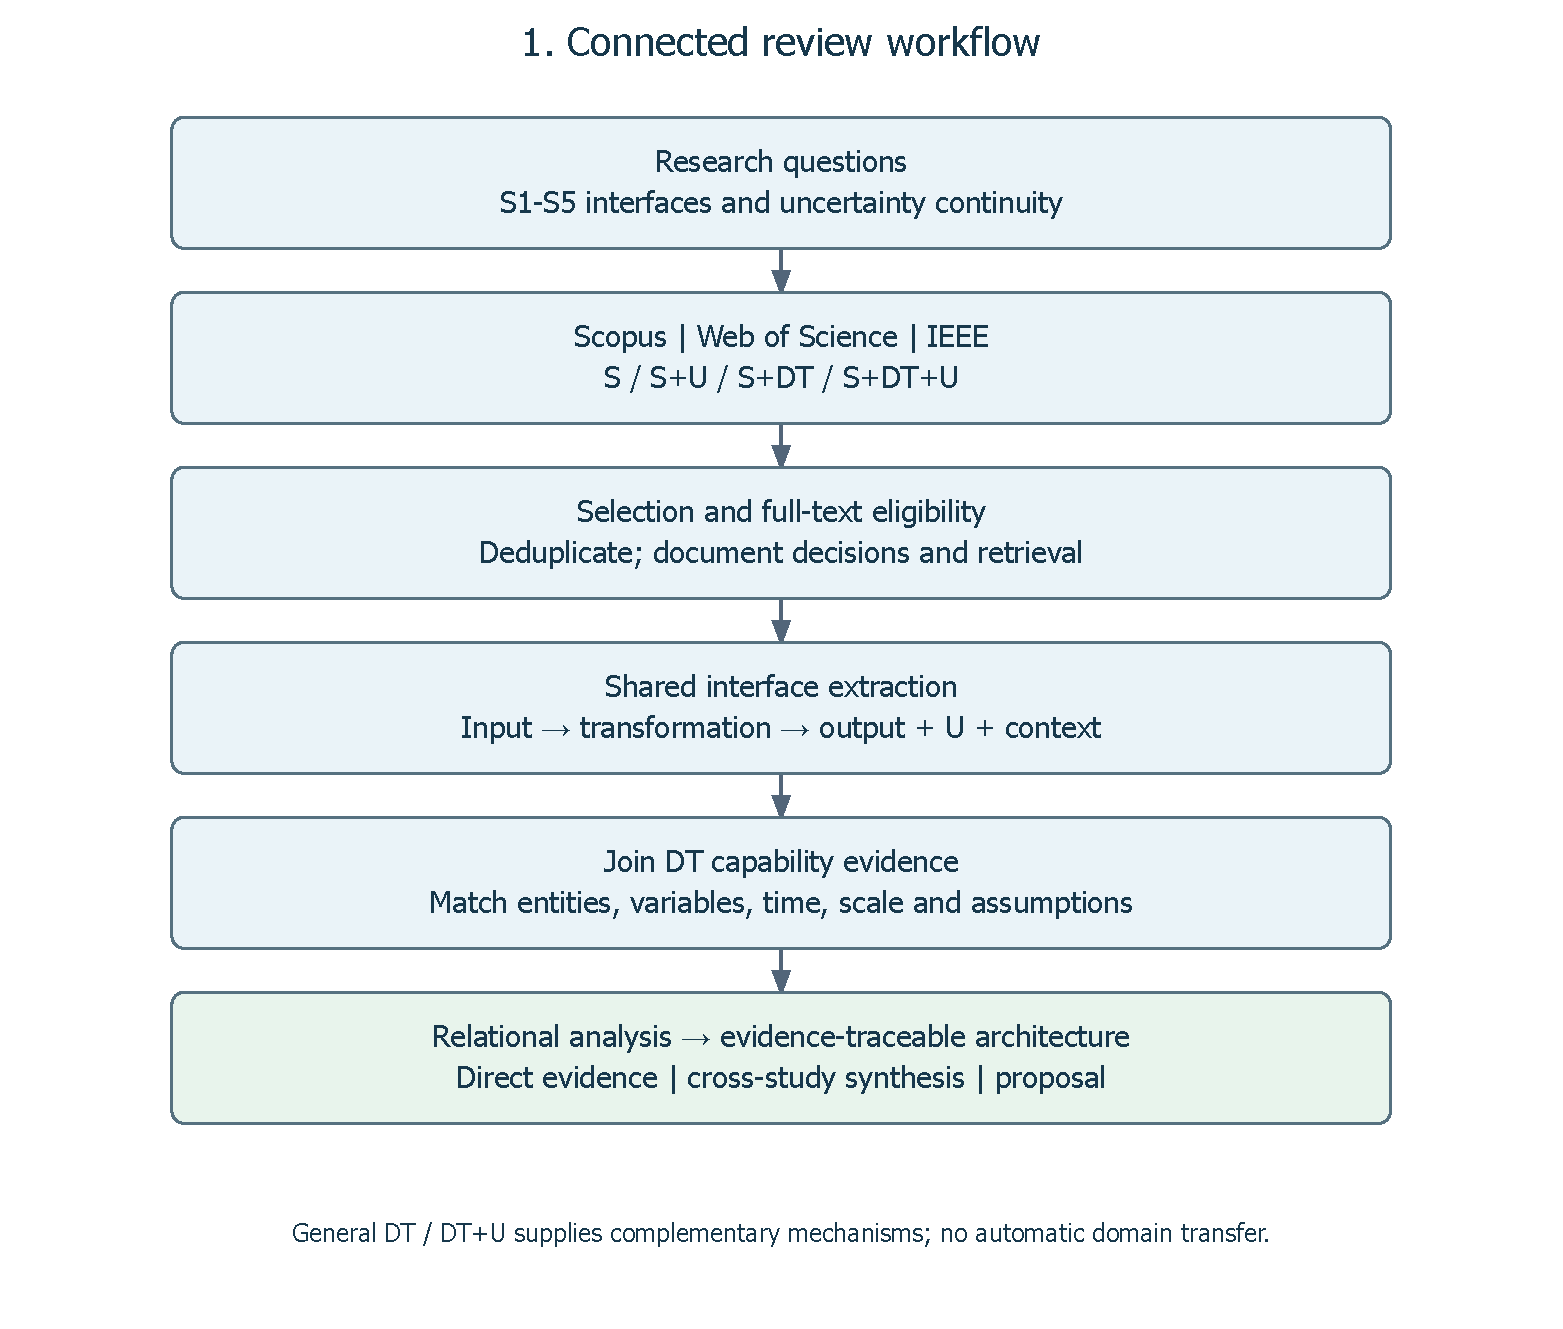
\includegraphics[width=\linewidth,height=.82\textheight,keepaspectratio]{../../figures/methods/workflow_en.pdf}\caption{Connected review workflow. Conceptual methodological design.}\end{figure}
\begin{figure}[p]\centering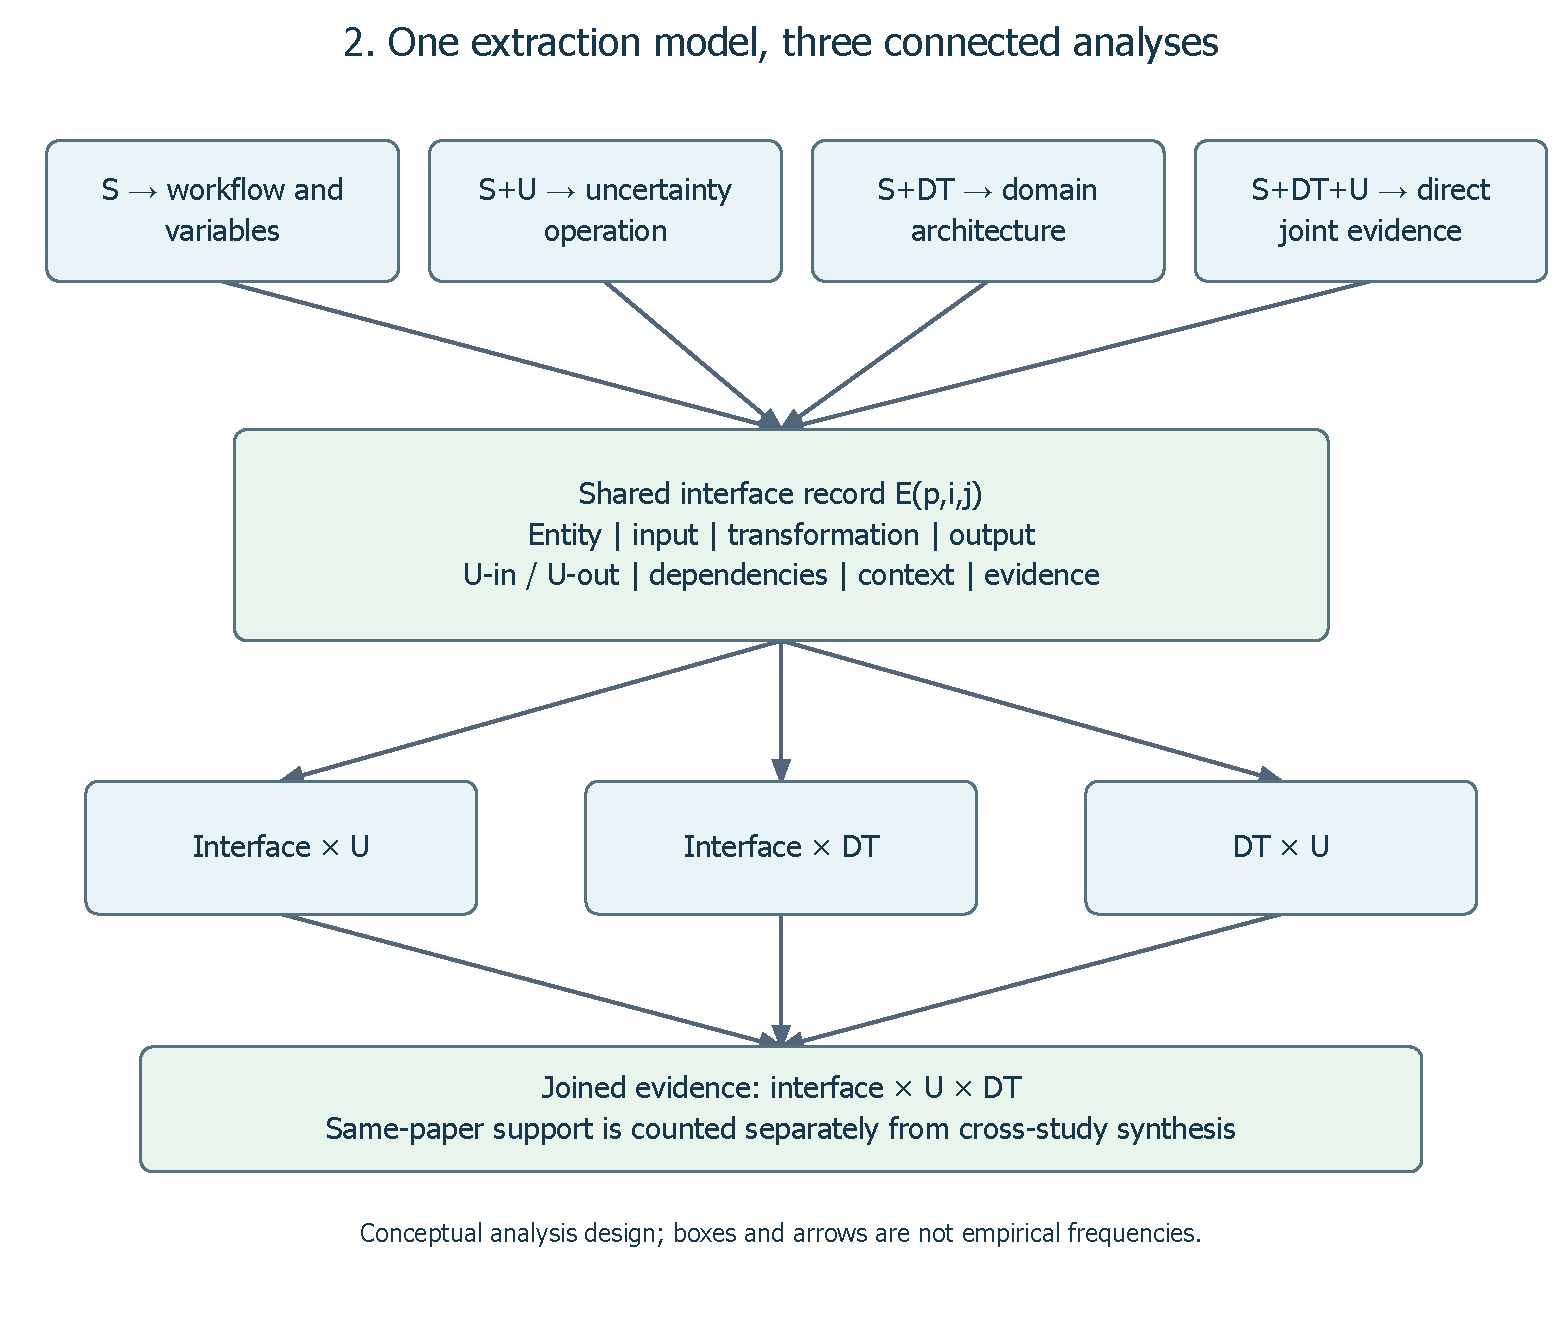
\includegraphics[width=\linewidth,height=.82\textheight,keepaspectratio]{../../figures/methods/evidence_join_en.pdf}\caption{Shared interface record and evidence joins.}\end{figure}
\begin{figure}[p]\centering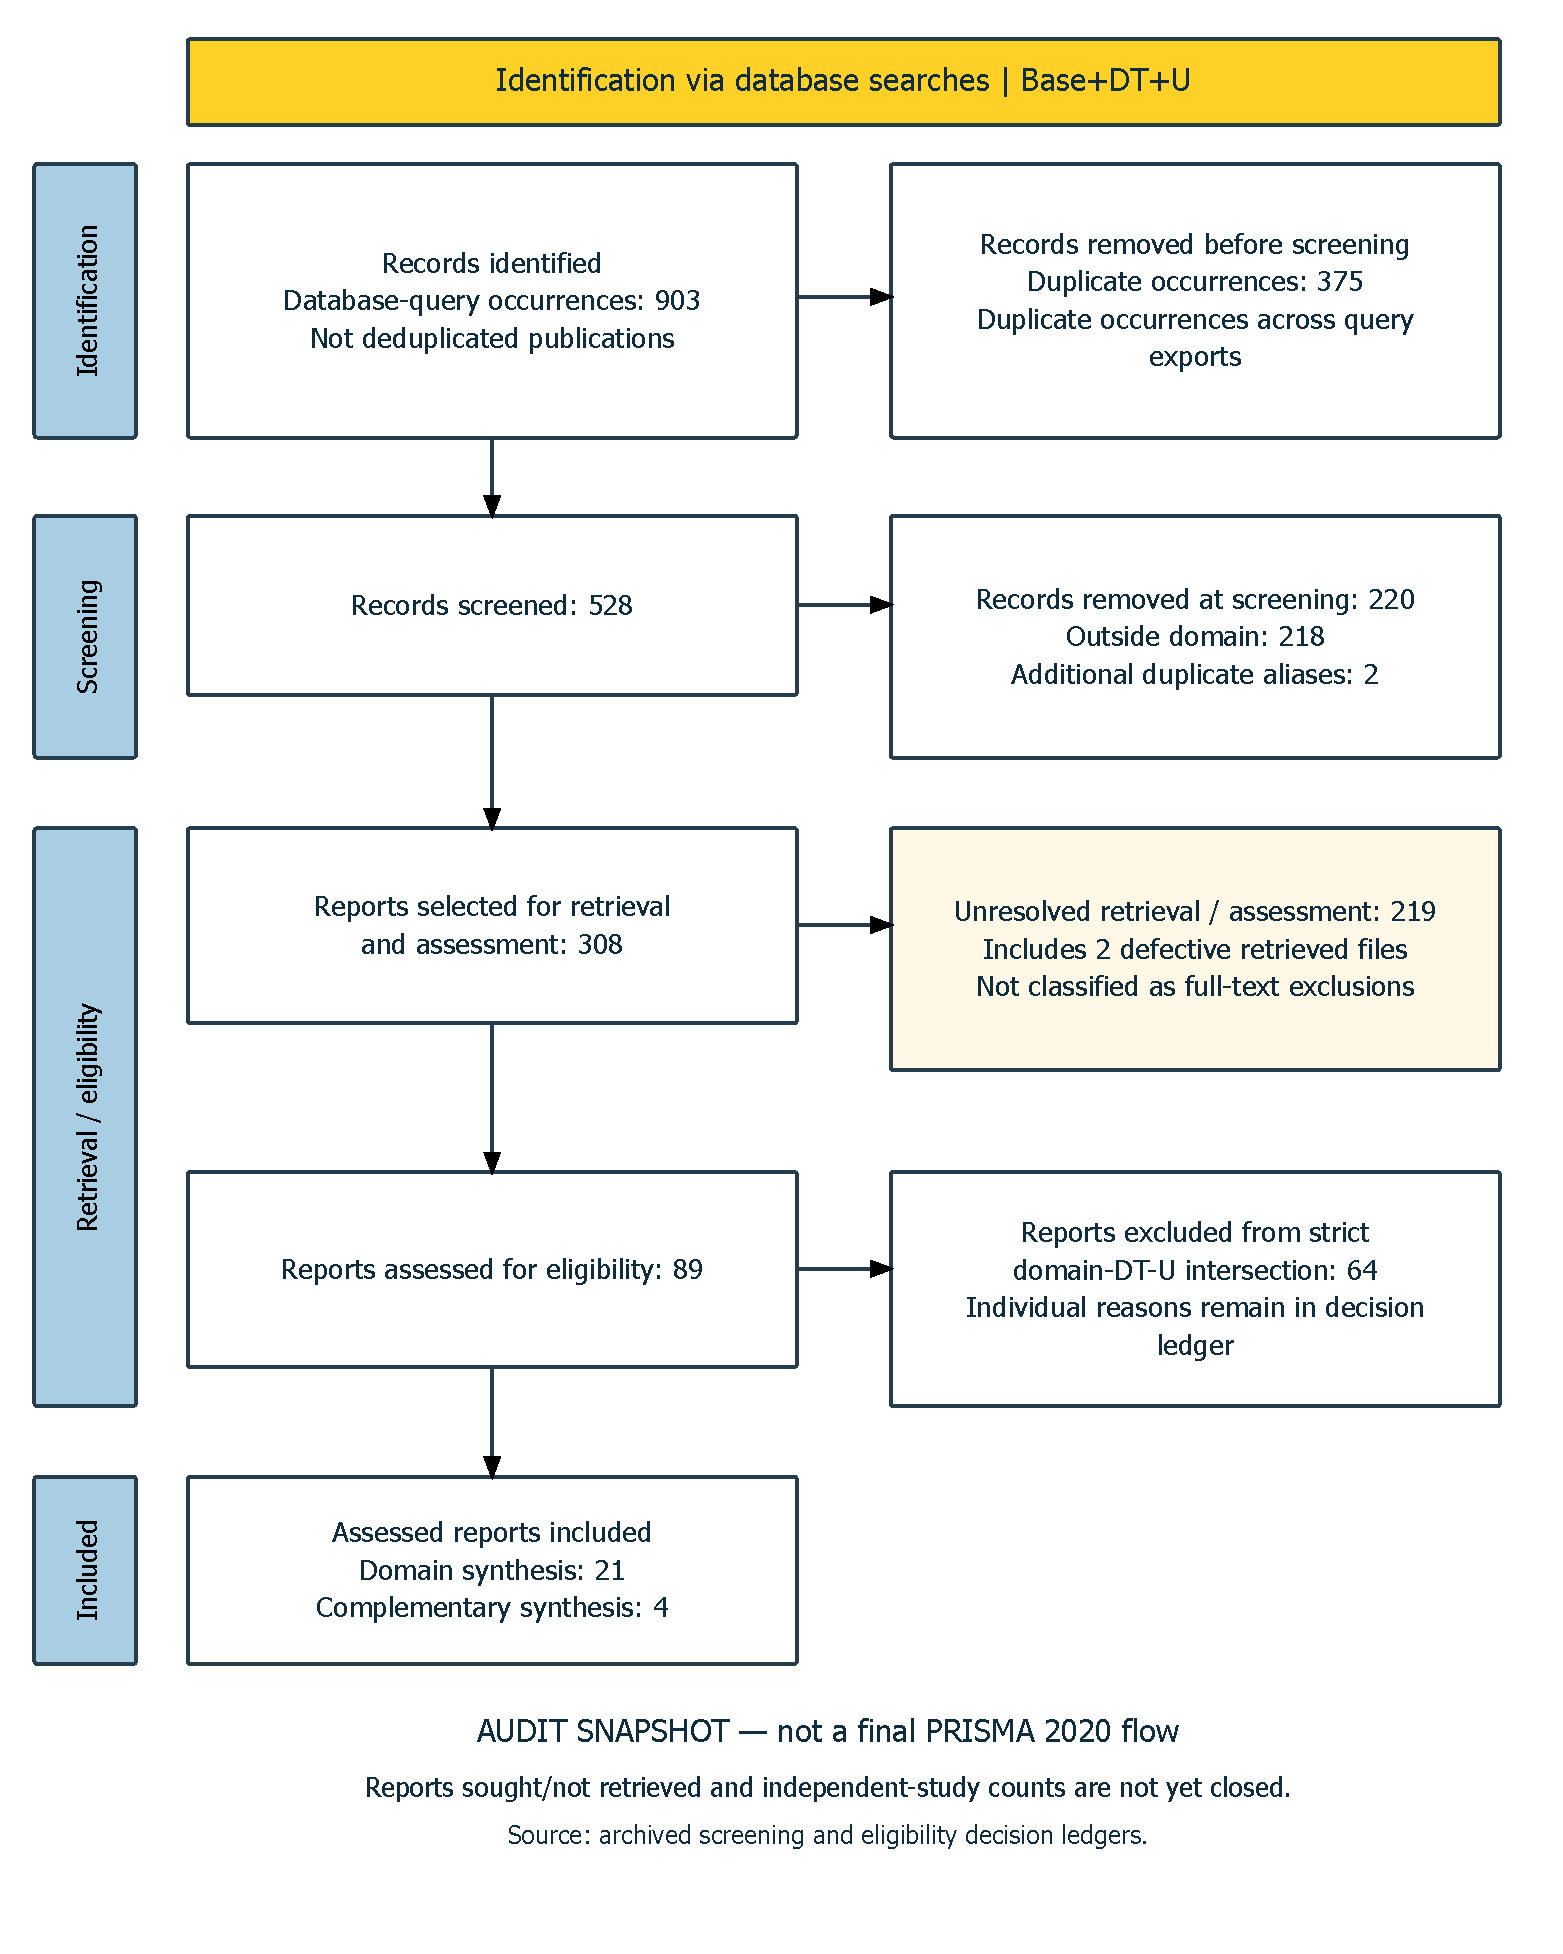
\includegraphics[width=\linewidth,height=.82\textheight,keepaspectratio]{../../figures/methods/prisma_broad_dtu_status_en.pdf}\caption{Broad Base+DT+U selection audit. Pending eligibility is not relabelled as exclusion.}\end{figure}
\begin{figure}[p]\centering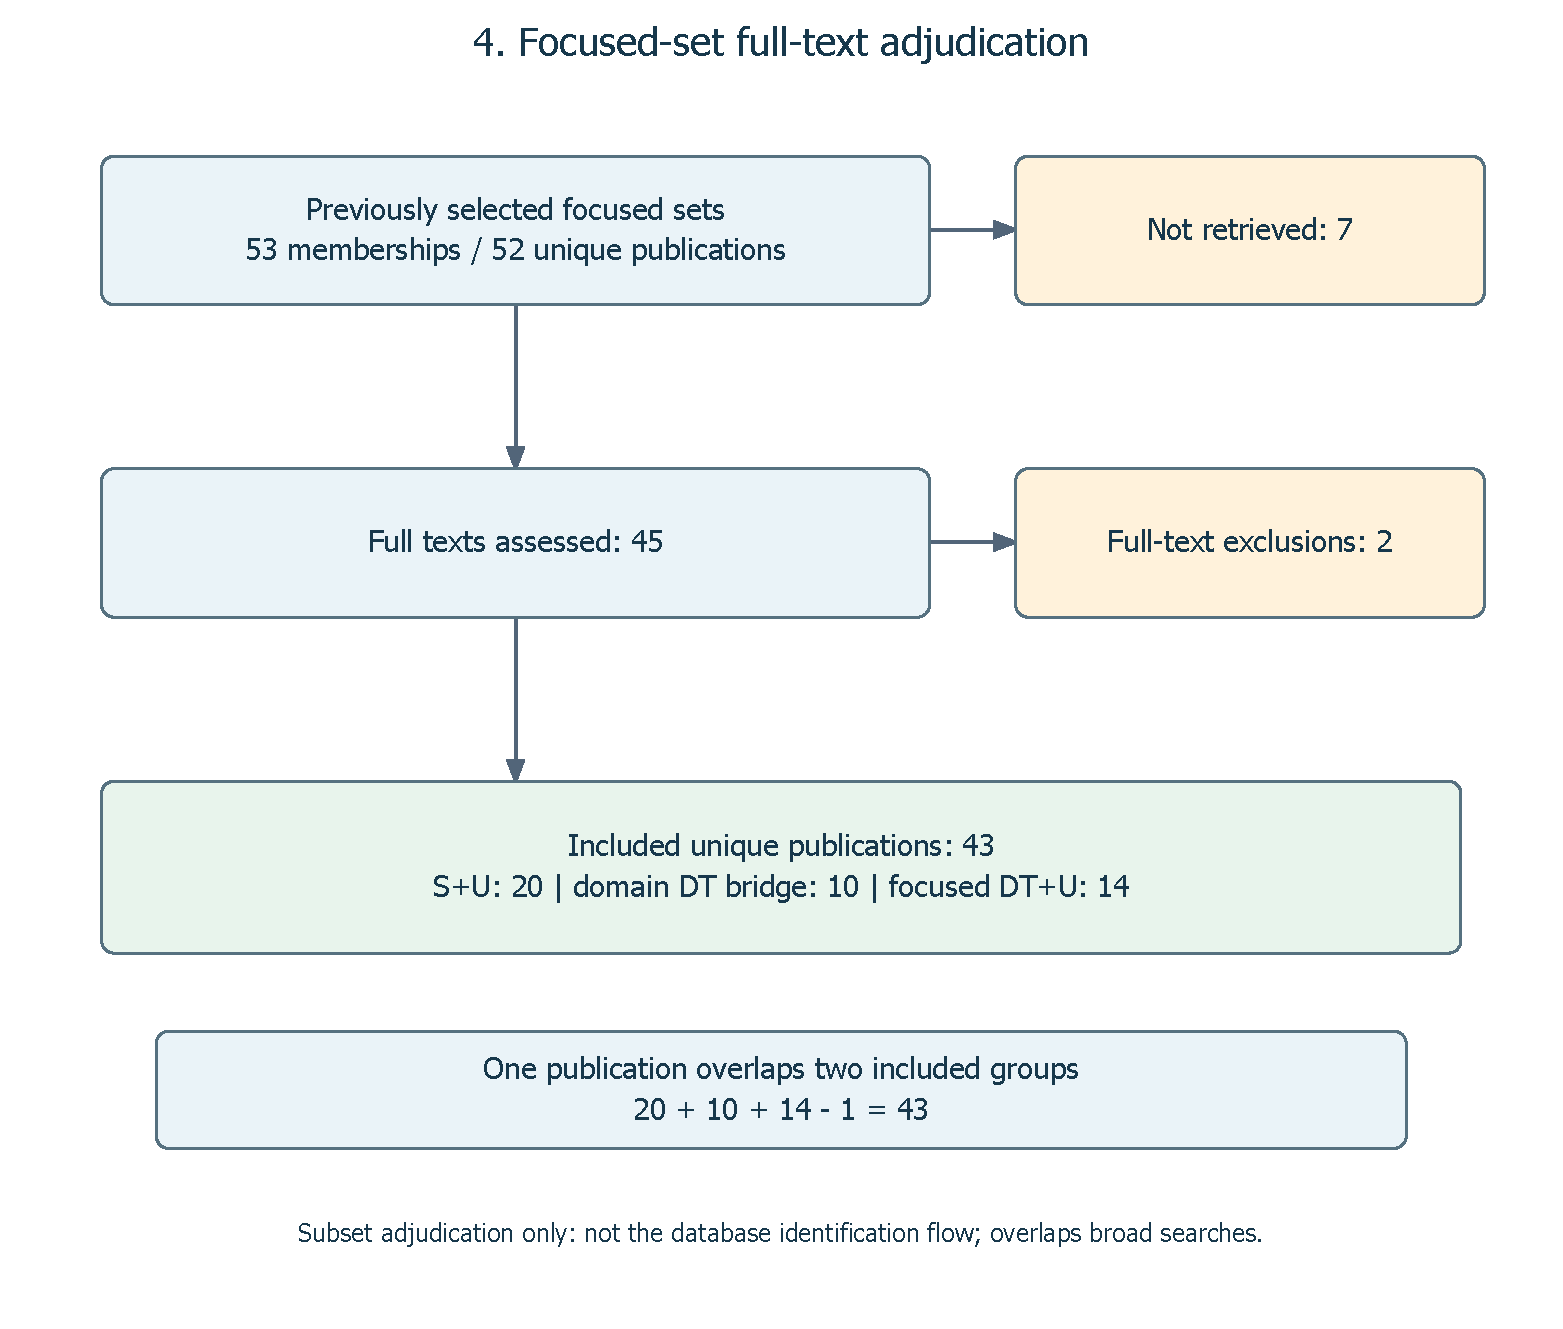
\includegraphics[width=\linewidth,height=.82\textheight,keepaspectratio]{../../figures/methods/focused_selection_status_en.pdf}\caption{Focused-set adjudication; overlapping subsets, not an additional independent database flow.}\end{figure}
\section{Results}
\subsection{Evidence sets and the meaning of the reported percentages}
The available analyses reveal an uneven connection between building information, material accounting and uncertainty-aware decisions. This finding emerges from several linked analytical subsets, rather than one interchangeable denominator. The archived S1–S3 analysis contains 17 publications with full-text or supporting-information-based coding. The current S+U relational analysis contains 20 publications contributing 23 assessed contexts. The domain DT function analysis contains nine publications with S1–S5 function codes; three adjacent-domain records are outside that graph. The general DT+U configuration analysis contains ten non-review publications. These sets support different questions and overlap in membership; their sizes must not be added to produce a review total.

All source and method percentages below were recalculated from article-level codes. Every one of the 17 legacy publications maps to an included publication in the current S+U eligibility ledger. This identity check establishes membership consistency, but does not independently validate every older interpretive code. The broader search remains incompletely adjudicated, as shown in the Methods selection diagrams. Accordingly, the reported distributions describe the named analytical subsets, not the prevalence of methods throughout the entire literature.

The percentages are frequencies of recorded evidence. For example, 64.7\% means that eleven of seventeen publications carry a particular source code. It does not mean that this source contributes 64.7\% of output variance. Similarly, the proportion of papers reporting Monte Carlo is not a measure of model accuracy, uncertainty magnitude or the effectiveness of uncertainty reduction.

\subsection{Sources, representations and downstream outcomes}
Material intensity/composition is the most frequent source in the legacy subset: 11/17 publications (64.7\%). Scenario/future context follows at 7/17 (41.2\%), temporal/event uncertainty at 6/17 (35.3\%), and model-form/structural uncertainty and LCA inventory/factor uncertainty each at 5/17 (29.4\%). Classification/prediction and hidden/missing building information each occur in 3/17 (17.6\%). Observation/measurement and transferability/domain shift each occur in 2/17 (11.8\%). Recovery/technical feasibility and boundary/allocation/accounting each occur in 1/17 (5.9\%). No positive spatial/logistics or demand/market-matching code is recorded in this subset. Those zeros delimit the extraction rather than establish that the wider research field ignores these problems.

The pattern places material representation and future assumptions at the centre of the observed uncertainty discussion. It also shows why a single label such as “data uncertainty” is insufficient: uncertain building attributes, material coefficients, lifetimes and environmental factors enter different transformations. Source categories do not automatically determine whether uncertainty is epistemic, aleatory or a mixture; that distinction depends on the model, observational support and decision context \citep{I25,U03,U11,U12}.

\begin{figure}[p]\centering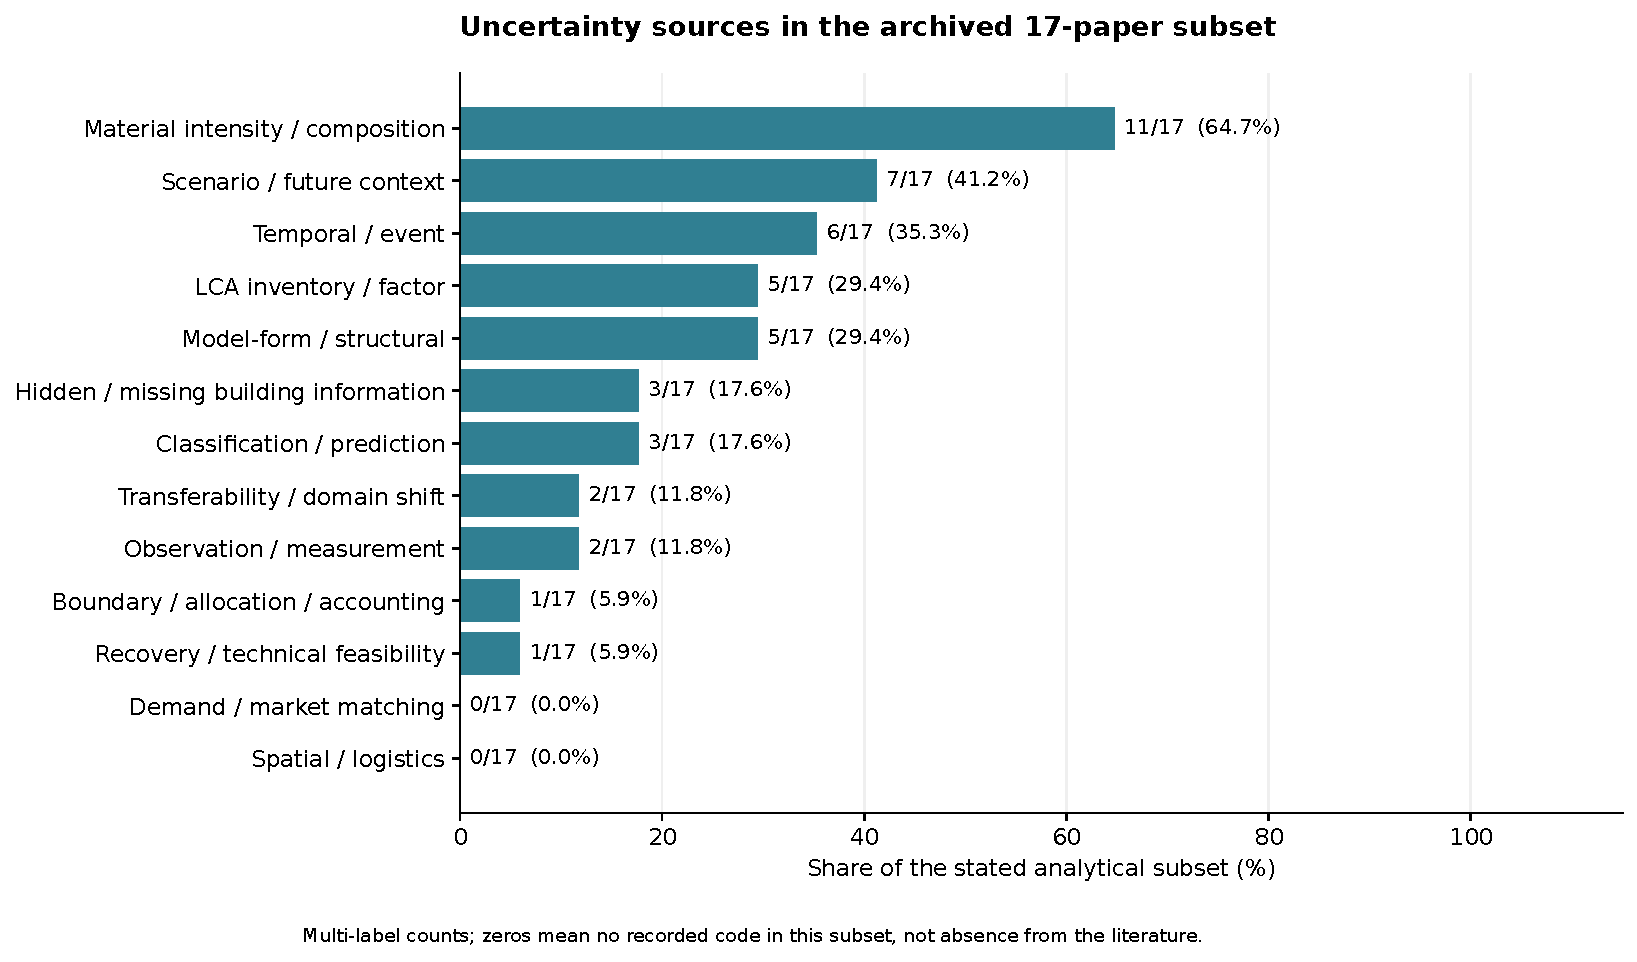
\includegraphics[width=\linewidth,height=.82\textheight,keepaspectratio]{../figures/F01_sources.pdf}\caption{Recalculated source frequencies, archived 17-paper coding. Multi-label, paper denominator.}\end{figure}
The legacy method codes record local/one-way sensitivity in 6/17 publications (35.3\%); scenario ensembles and bootstrap each in 4/17 (23.5\%); ranges/intervals and Monte Carlo each in 3/17 (17.6\%); and probabilistic ML/parameter modelling in 2/17 (11.8\%). Three publications (17.6\%) carry the legacy deterministic/no-formal-UQ category. No positive Bayesian, global-sensitivity, fuzzy/possibility or analytical-error-propagation code is recorded. These are broad inherited categories: bootstrap used for training-data augmentation is not equivalent to bootstrap used to estimate an output interval, and a probability distribution assigned to an input is not proof that it was propagated. The more specific context coding used in D04 retains these functional distinctions.

\begin{figure}[p]\centering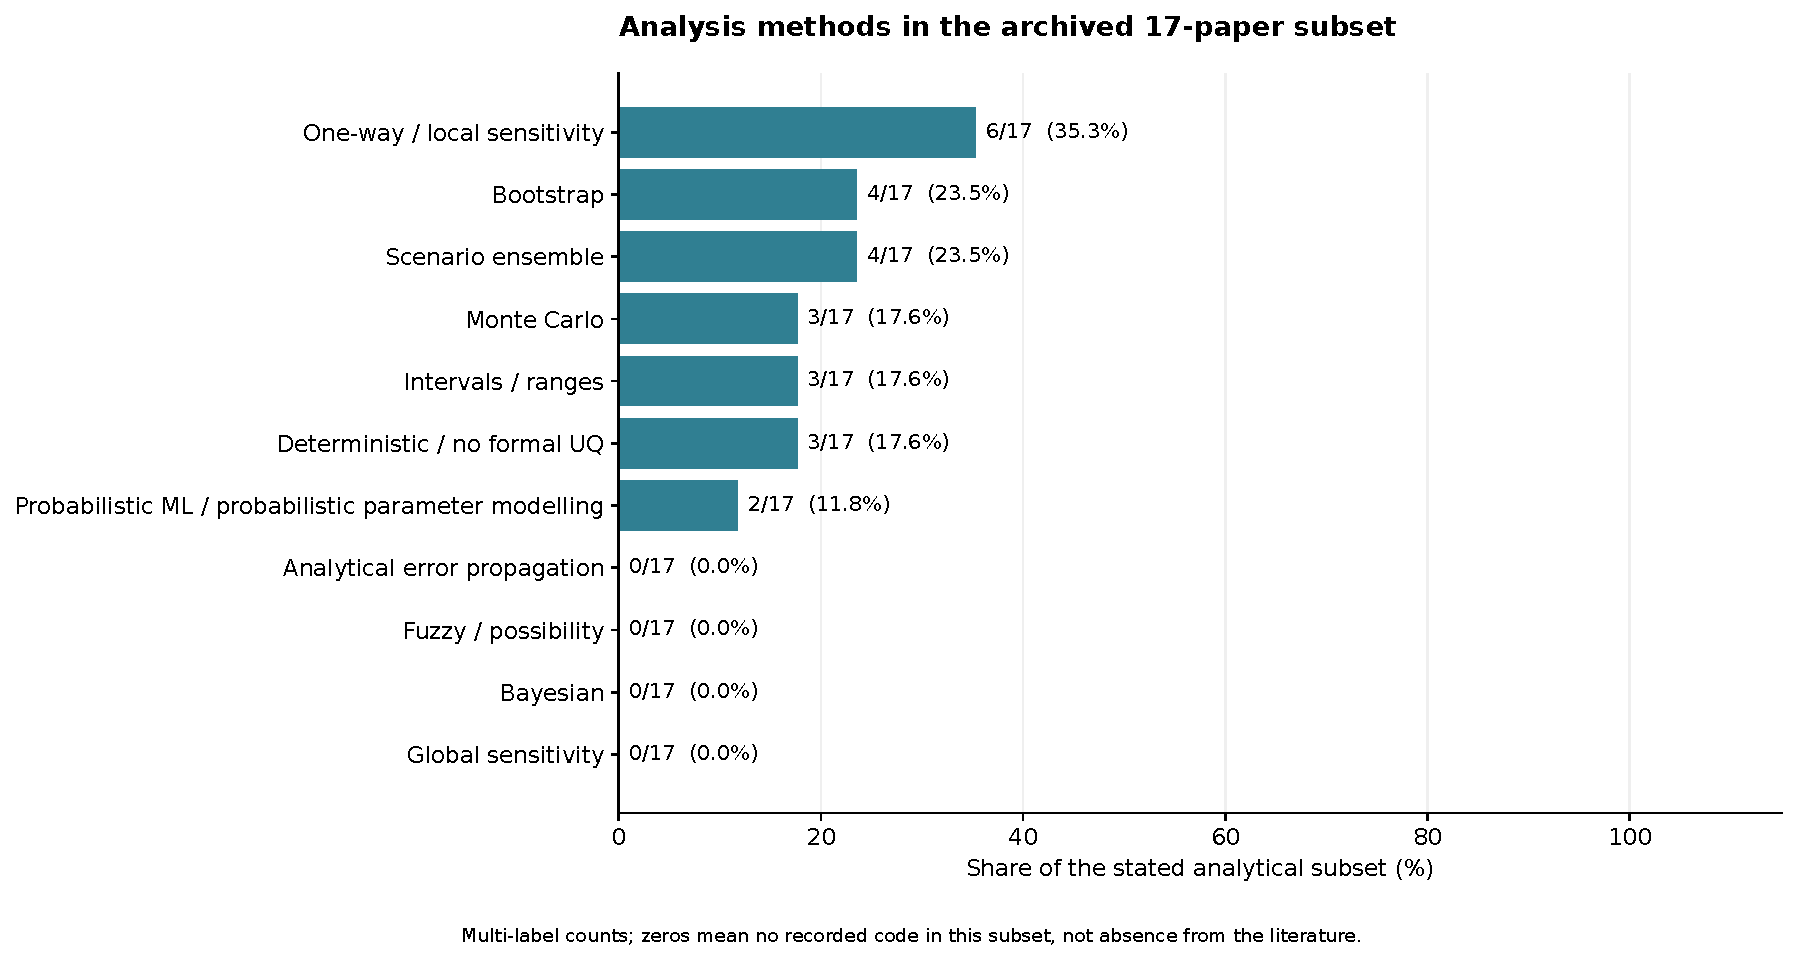
\includegraphics[width=\linewidth,height=.82\textheight,keepaspectratio]{../figures/F02_methods.pdf}\caption{Recalculated method frequencies in the same 17 papers; broad legacy codes retain their original scope.}\end{figure}
The six legacy downstream-outcome labels are also reproducible: unassessed in 9/17 publications (52.9\%); transformed in 7/17 (41.2\%); preserved and masked/lost each in 3/17 (17.6\%); and amplified and legitimately reduced each in 1/17 (5.9\%). Labels overlap because a publication may examine several boundaries or operations. In particular, a paper can analyse downstream parameter variability while leaving uncertainty from upstream inference unassessed. The outcome percentages therefore do not sum to 100\%.

The frequency labels should be interpreted at the strength of their underlying evidence. The single amplified/reduced case concerns sensitivity to lifetime assumptions and spatial aggregation \citep{U11}; it does not establish that a DT reduced real uncertainty. Likewise, “transformed” can denote a change in the representation or consequences of variability, not necessarily an estimated upstream and downstream probability density. The conceptual distribution sketches make the distinctions legible, but no curve in those sketches is fitted to the reviewed studies.

\begin{figure}[p]\centering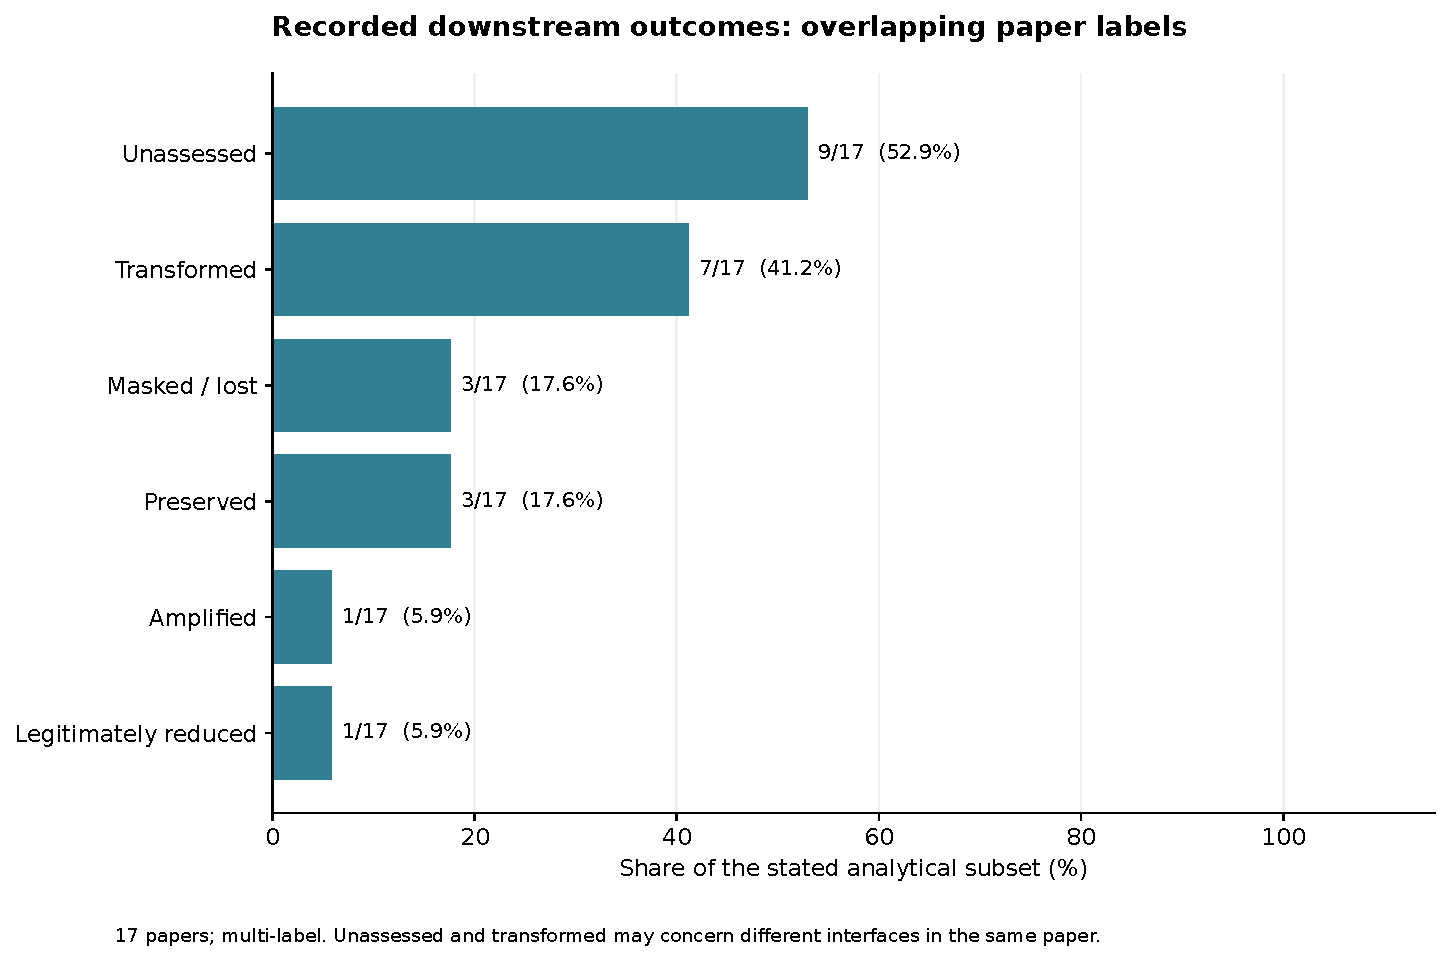
\includegraphics[width=\linewidth,height=.82\textheight,keepaspectratio]{../figures/F03_outcomes.pdf}\caption{Legacy outcome labels reconstructed with supporting IDs. These are not measured variance changes.}\end{figure}
\begin{figure}[p]\centering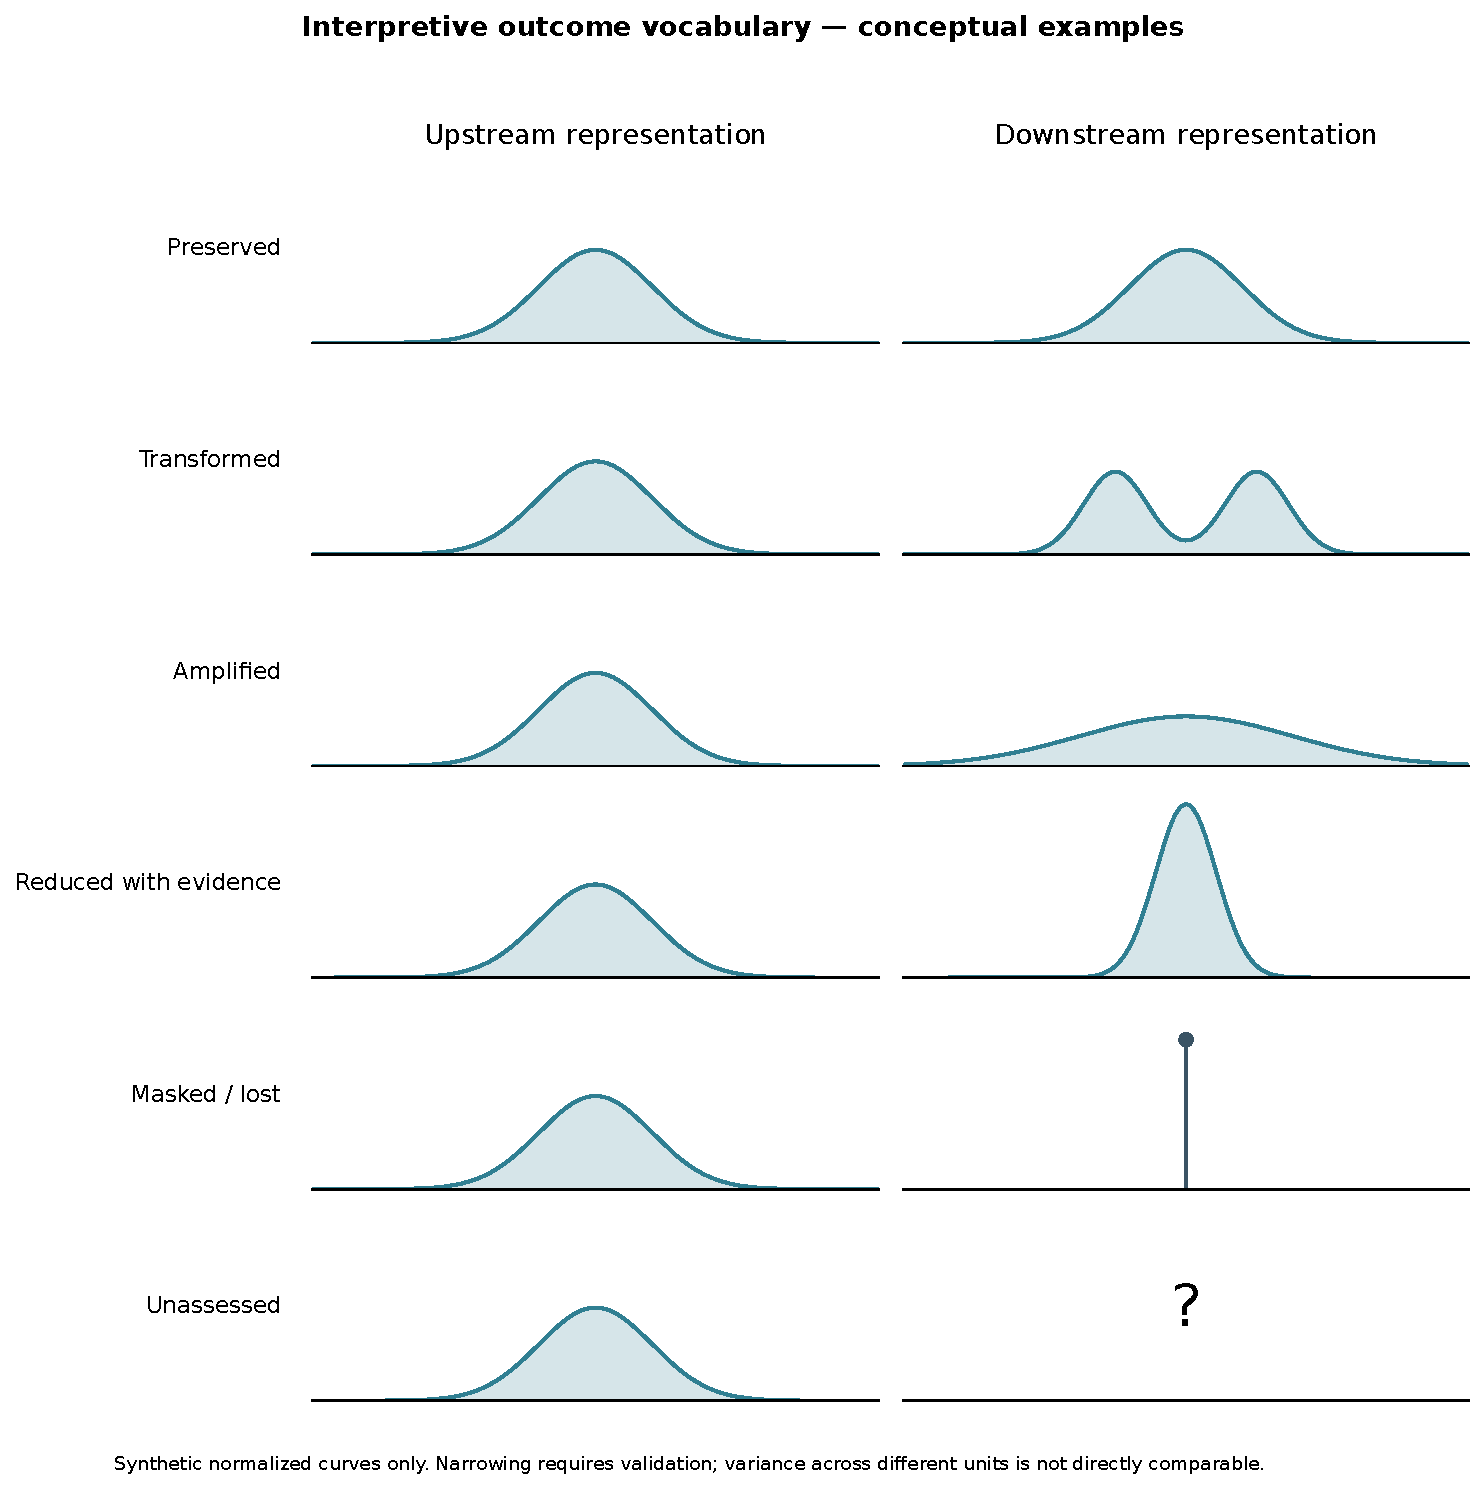
\includegraphics[width=\linewidth,height=.82\textheight,keepaspectratio]{../figures/F06_outcome_vocabulary.pdf}\caption{Conceptual outcome vocabulary. Synthetic normalized curves; not data from the reviewed models.}\end{figure}
\subsection{Where continuity is documented across the four boundaries}
The current boundary coding separates evidence of an uncertain input from evidence of its downstream treatment. At S1→S2, nine contexts are assessed. Four (44.4\%) do not demonstrate downstream transfer; two (22.2\%) provide sensitivity/representation comparisons; one each (11.1\%) provides review/discussion, prepares inputs for propagation, or documents partial transfer. None is coded as quantified output uncertainty for selected inputs in this boundary-specific classification. Material-intensity distributions and prediction-error measures can therefore improve the input description without establishing a complete uncertain stock estimate \citep{U03,U04,U05}.

At S2→S3, six contexts are assessed: three (50.0\%) document partial transfer, two (33.3\%) quantify outputs for selected uncertain inputs, and one (16.7\%) does not demonstrate transfer. The stronger evidence here is consistent with the explicit use of lifetime distributions, probabilistic parameters and dynamic material-flow models \citep{U11,U12,U13,U18}. However, an uncertain lifetime model can coexist with deterministic upstream quantities. The evidence does not justify interpreting the entire chain as probabilistic simply because the stock-dynamics calculation uses sampling.

No S3→S4 context is assessed in this particular harmonised coding set. A percentage is therefore undefined, rather than zero percent successful propagation. The sole S4→S5 context is coded as partial transfer: 1/1, or 100\% of one observation. This is a case description, not a stable estimate of methodological prevalence \citep{U19}. Seven additional contexts concern other inputs to S5. They remain separate because environmental-factor, damage or emissions analyses do not necessarily consume material-recovery outputs. Reassigning them to S4→S5 would create continuity that the extraction has not established \citep{U15,U16,U20,U21}.

\begin{figure}[p]\centering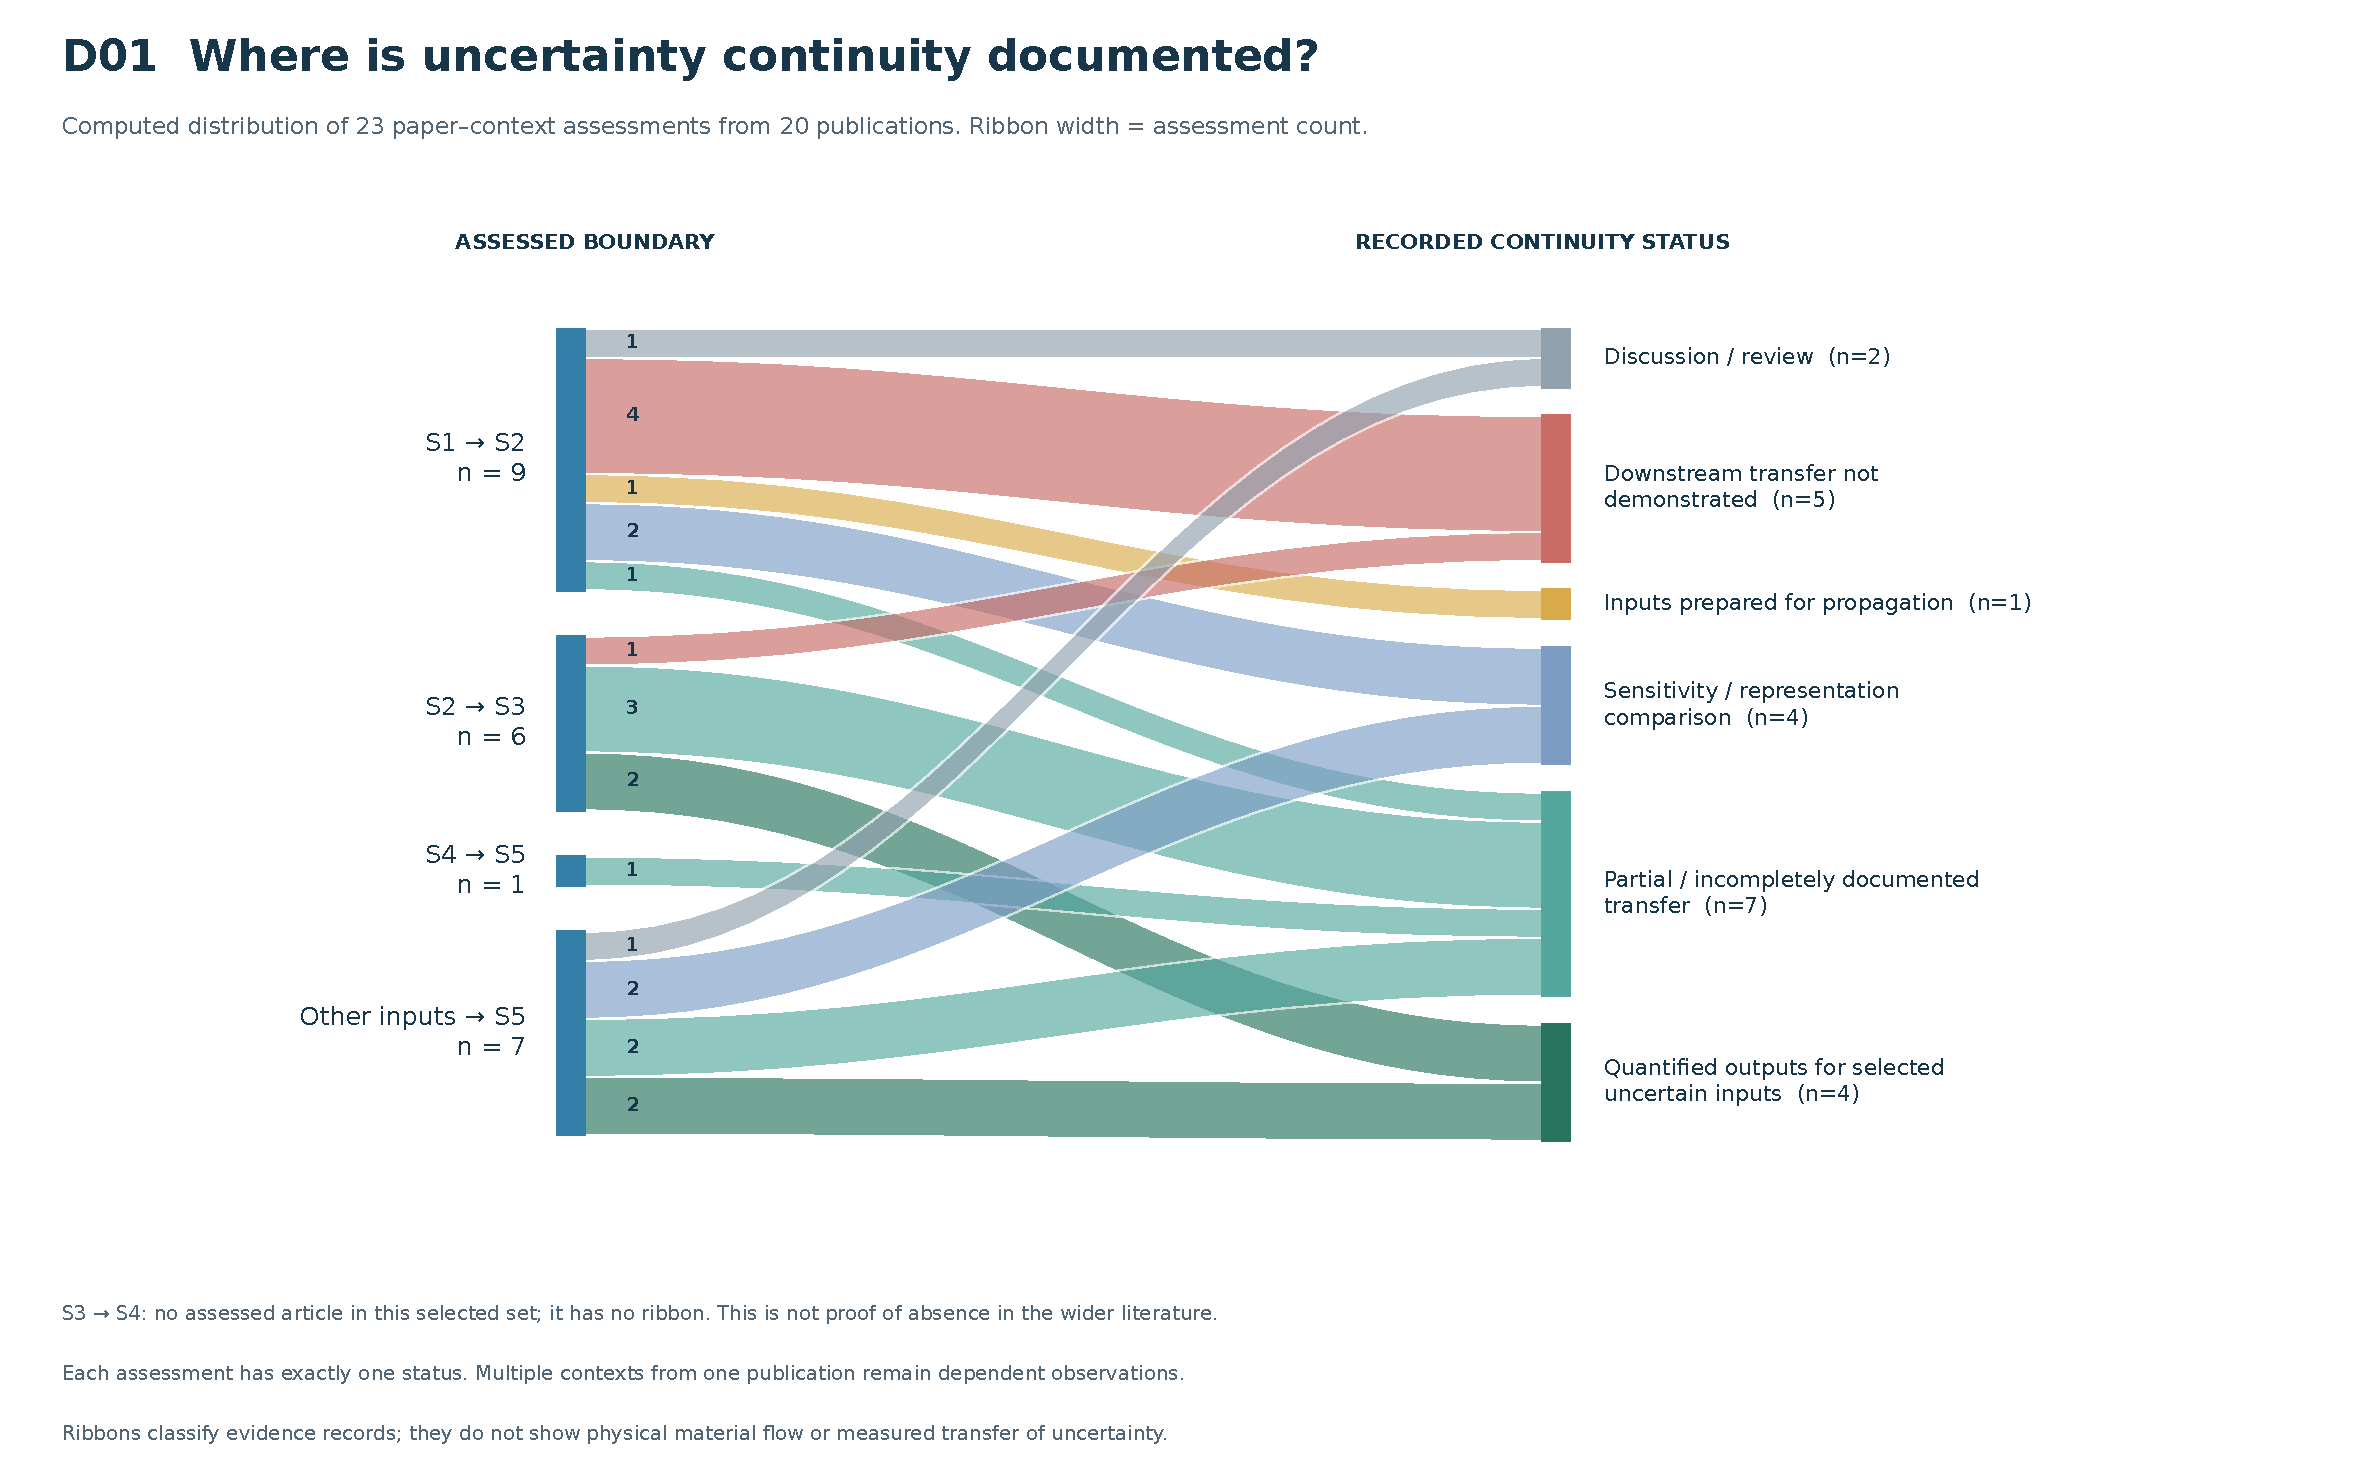
\includegraphics[width=\linewidth,height=.82\textheight,keepaspectratio]{../../relational_analysis/data_diagrams/figures/D01_boundary_continuity_alluvial.pdf}\caption{Current boundary–continuity coding: 23 contexts from 20 publications.}\end{figure}
\begin{figure}[p]\centering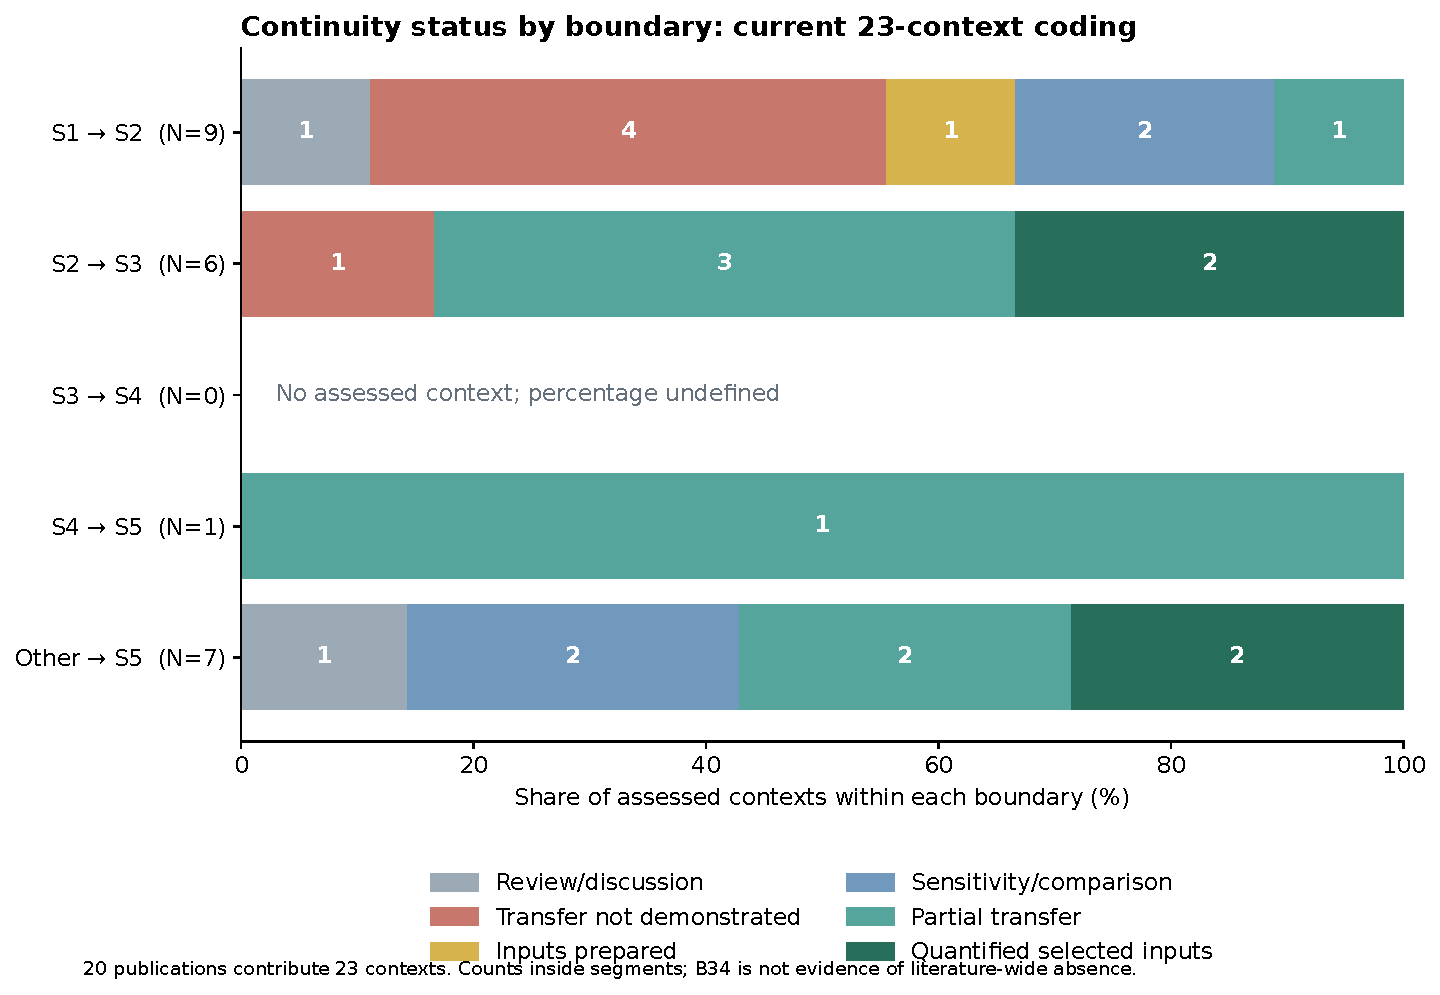
\includegraphics[width=\linewidth,height=.82\textheight,keepaspectratio]{../figures/F04_boundary_percentages.pdf}\caption{Within-boundary percentages and counts. B34 denominator is zero, so its percentage is undefined.}\end{figure}
The distribution across all 23 contexts is seven partial-transfer assessments (30.4\%), five without demonstrated downstream transfer (21.7\%), four sensitivity/comparison assessments and four quantified-selected-input assessments (17.4\% each), two review/discussion assessments (8.7\%), and one propagation-ready assessment (4.3\%). These categories are mutually exclusive within a context, but the contexts are not independent studies. The classification differs deliberately from the legacy six-outcome labels: it grades what the extraction demonstrates about an interface, rather than inferring the physical fate of every uncertainty component.

\subsection{Which DT functions and uncertainty mechanisms are recorded?}
Within the nine domain-function records, seven publications have a positive S1 function code and seven have a positive S2 code (77.8\% each). S3 and S4 each have two (22.2\%), and S5 has one (11.1\%). A publication may contribute to several stages. The weighted network contains sixteen positive stage–function combinations. Observation/inference, semantic material information, identity/provenance and inventory modelling dominate the recorded architecture. Presence at two stages does not establish an operational connection between them; the graph is a functional coverage map, not a measured uncertainty-transfer network.

\begin{figure}[p]\centering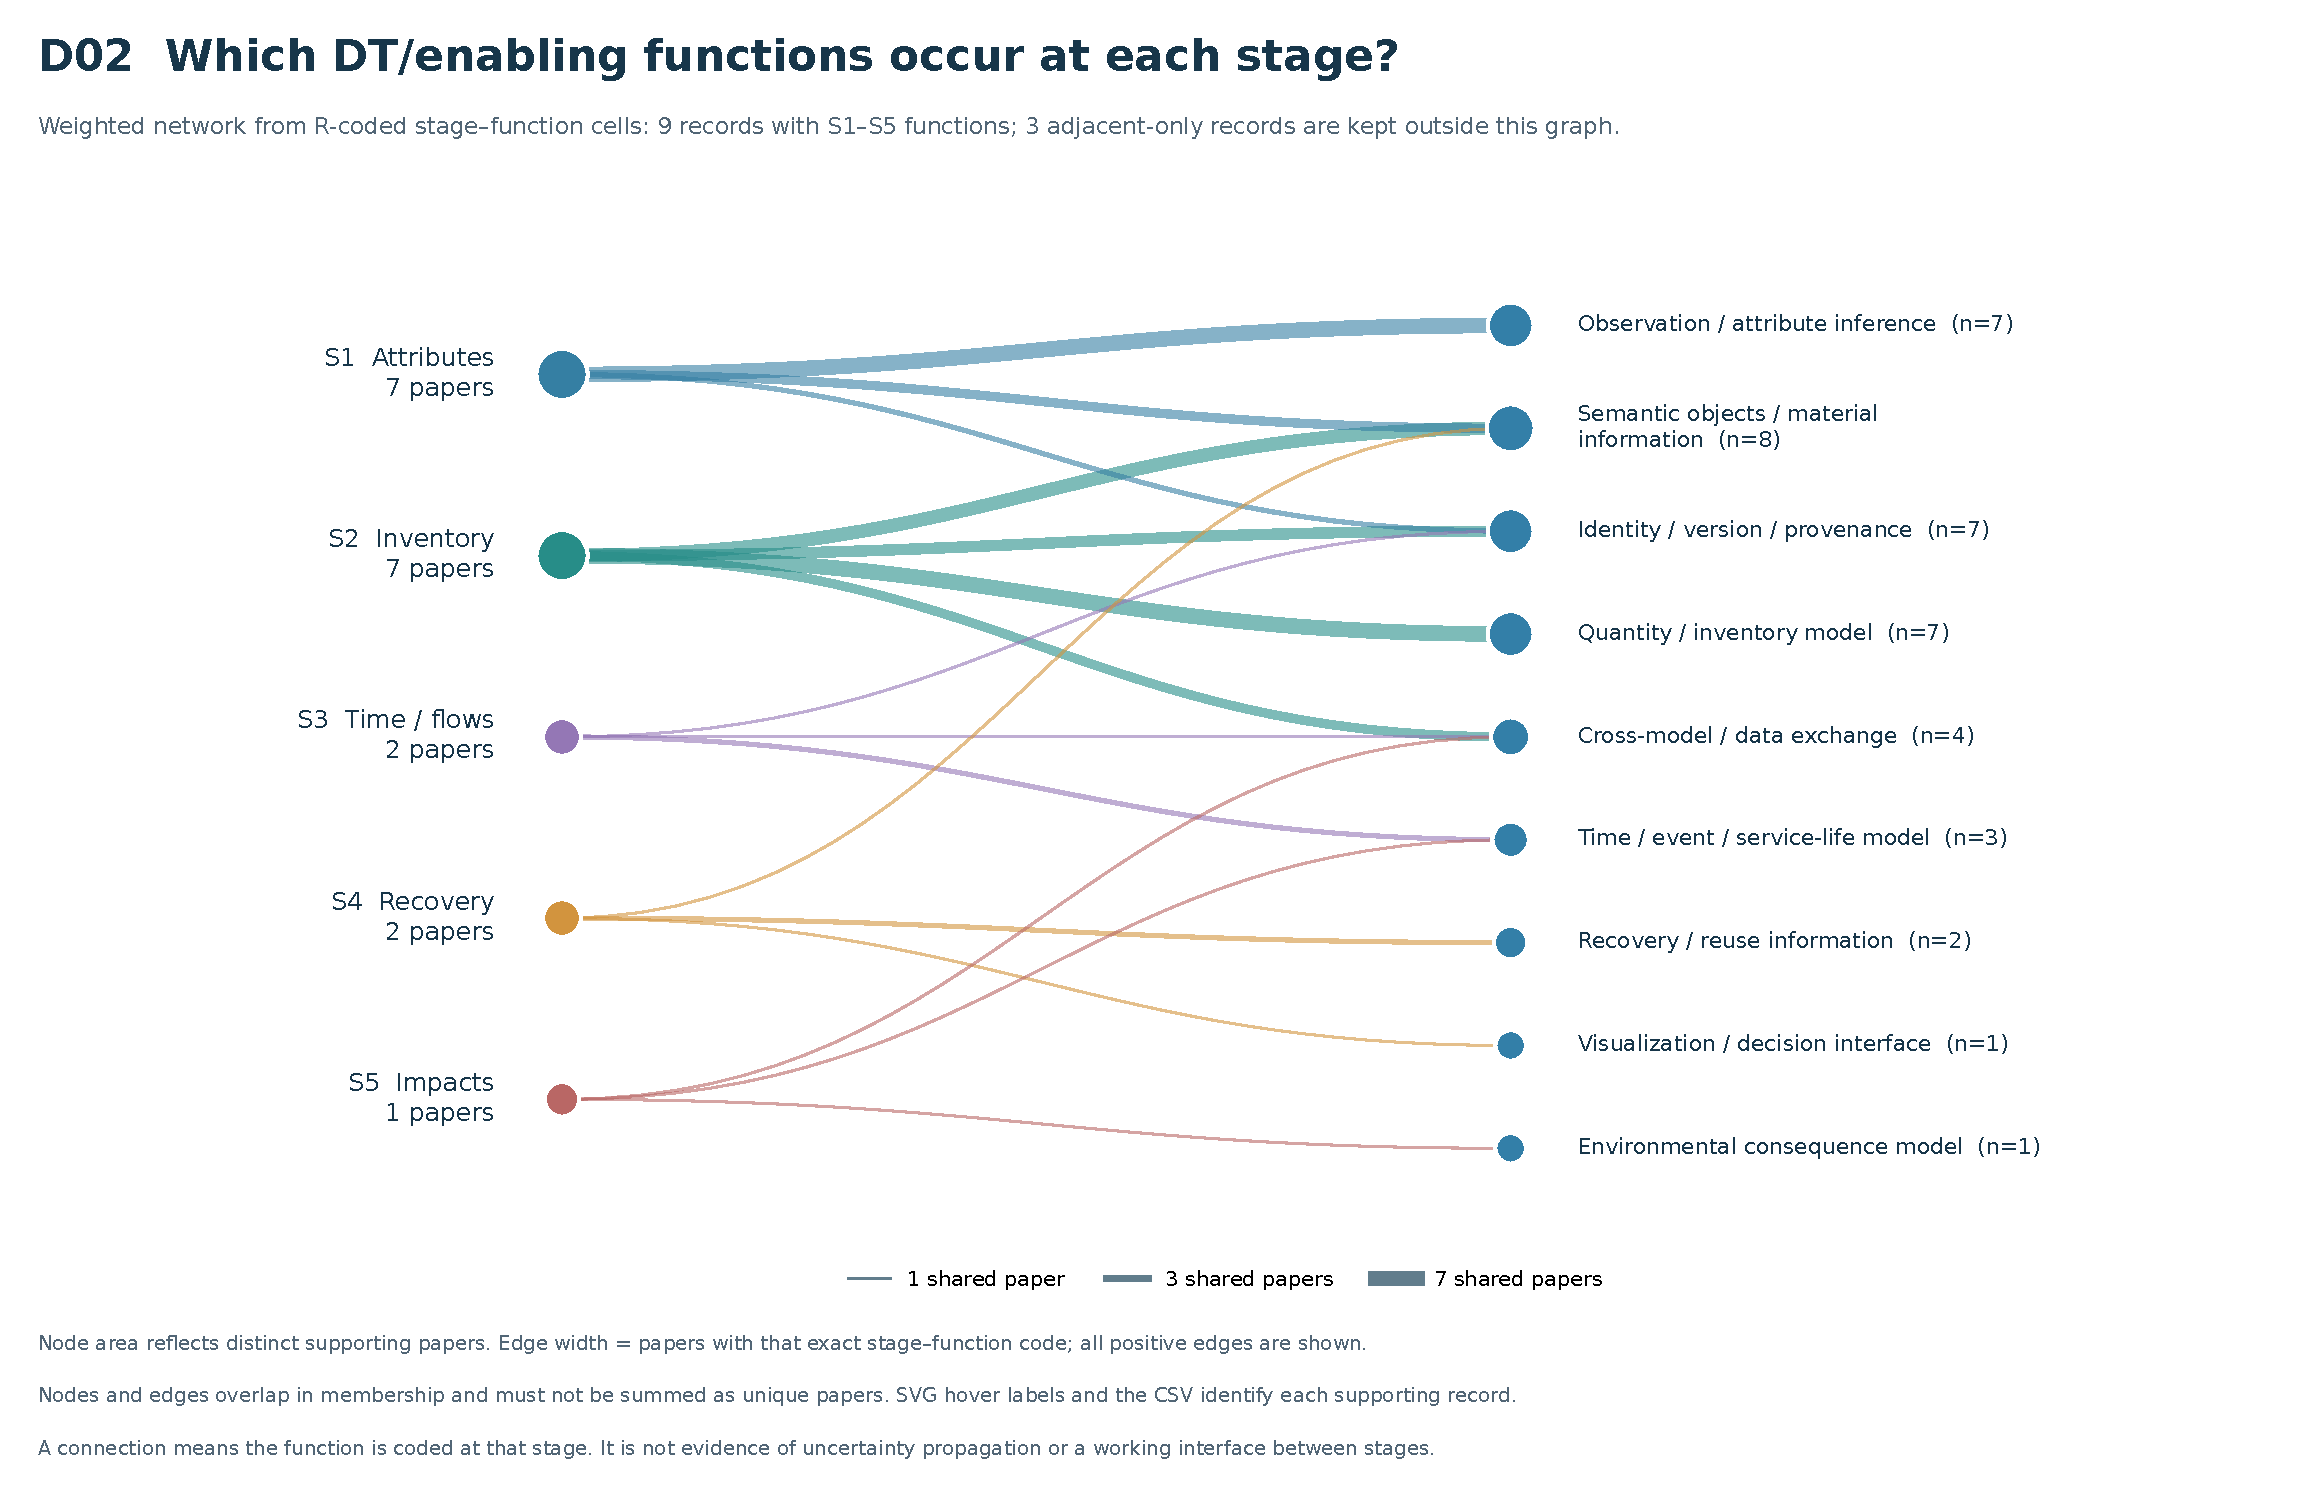
\includegraphics[width=\linewidth,height=.82\textheight,keepaspectratio]{../../relational_analysis/data_diagrams/figures/D02_stage_function_network.pdf}\caption{Stage–function co-coding; edge width is distinct supporting publications, not uncertainty flow.}\end{figure}
The ten non-review general DT+U records show a different emphasis. Probabilistic uncertainty representation and residual/shift diagnostics each appear in eight records (80\%). Bayesian state/parameter inference, online adaptation and uncertainty-linked alerts/actions each appear in seven (70\%). Empirical interval-coverage assessment appears in three (30\%), and explicit joint/dependence transport in two (20\%). These percentages refer to recorded positive method descriptions. They neither establish successful deployment in circular construction nor prove that an unrecorded feature was absent from the implementation.

Nine exact positive-code configurations occur across the ten records. One configuration is shared by two papers; the remaining eight occur once each. This heterogeneity supports a vocabulary of composable capabilities, rather than one empirically dominant DT architecture. Especially relevant to continuity is the difference between frequently recorded prediction/update capabilities and less frequently recorded joint-dependence transport. A system can update a model and issue an alert while still losing upstream correlation information at the next model interface.

\begin{figure}[p]\centering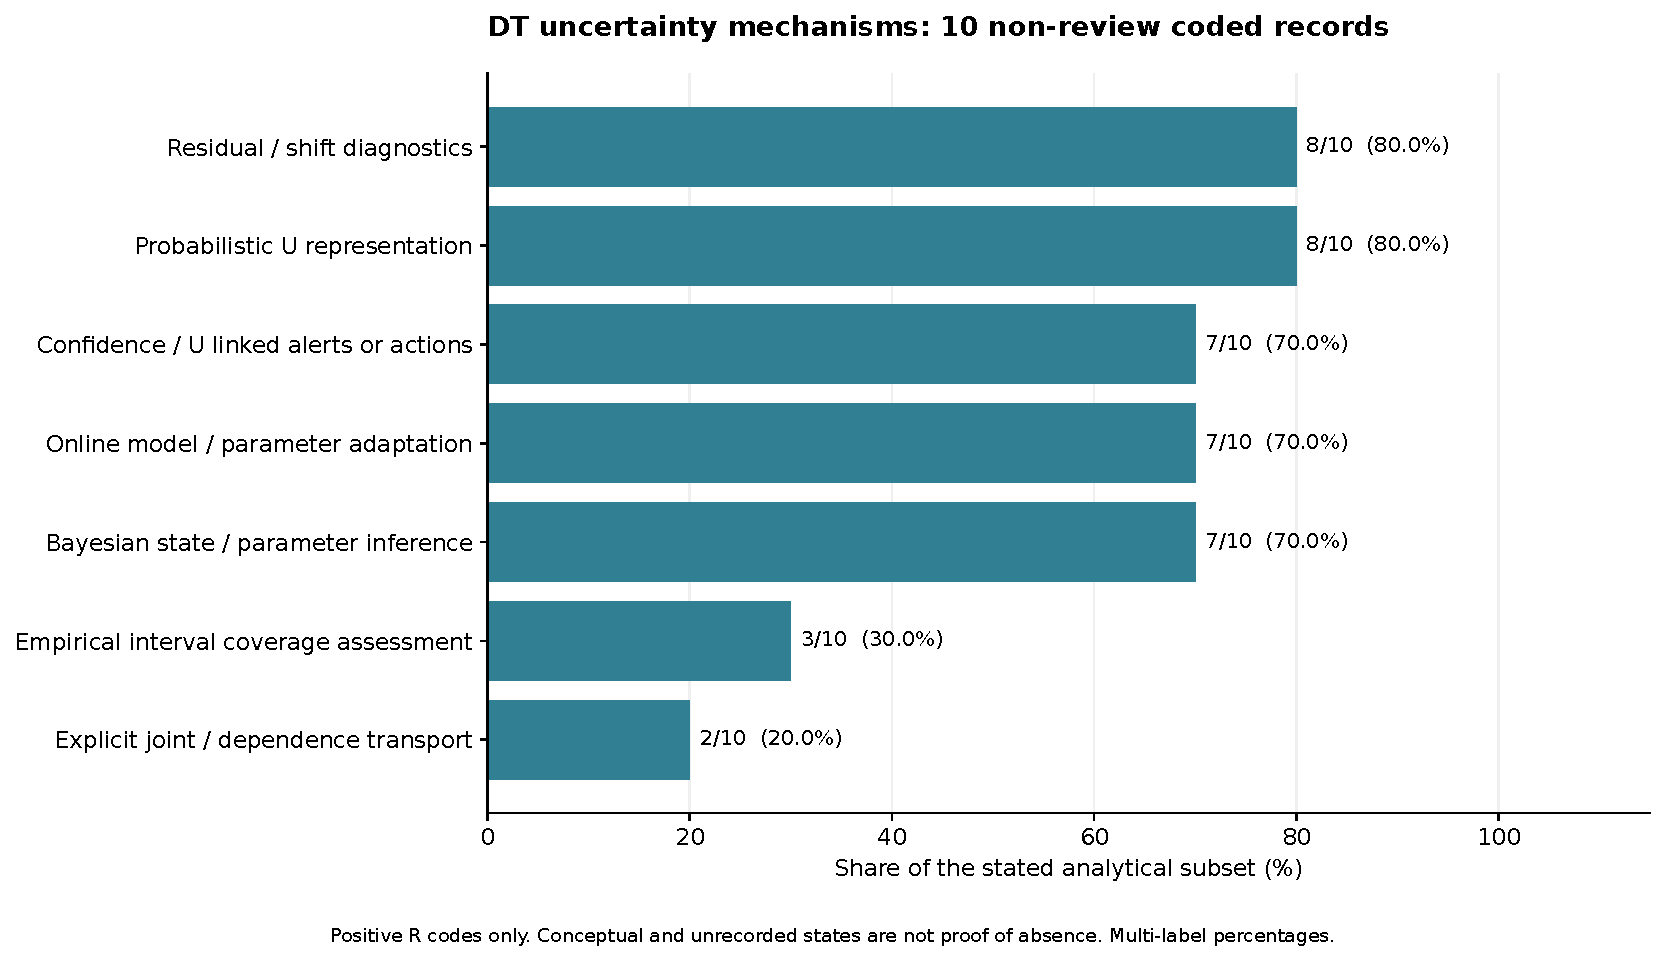
\includegraphics[width=\linewidth,height=.82\textheight,keepaspectratio]{../figures/F05_dt_mechanisms.pdf}\caption{Positive mechanism frequency in ten non-review general-DT records.}\end{figure}
\begin{figure}[p]\centering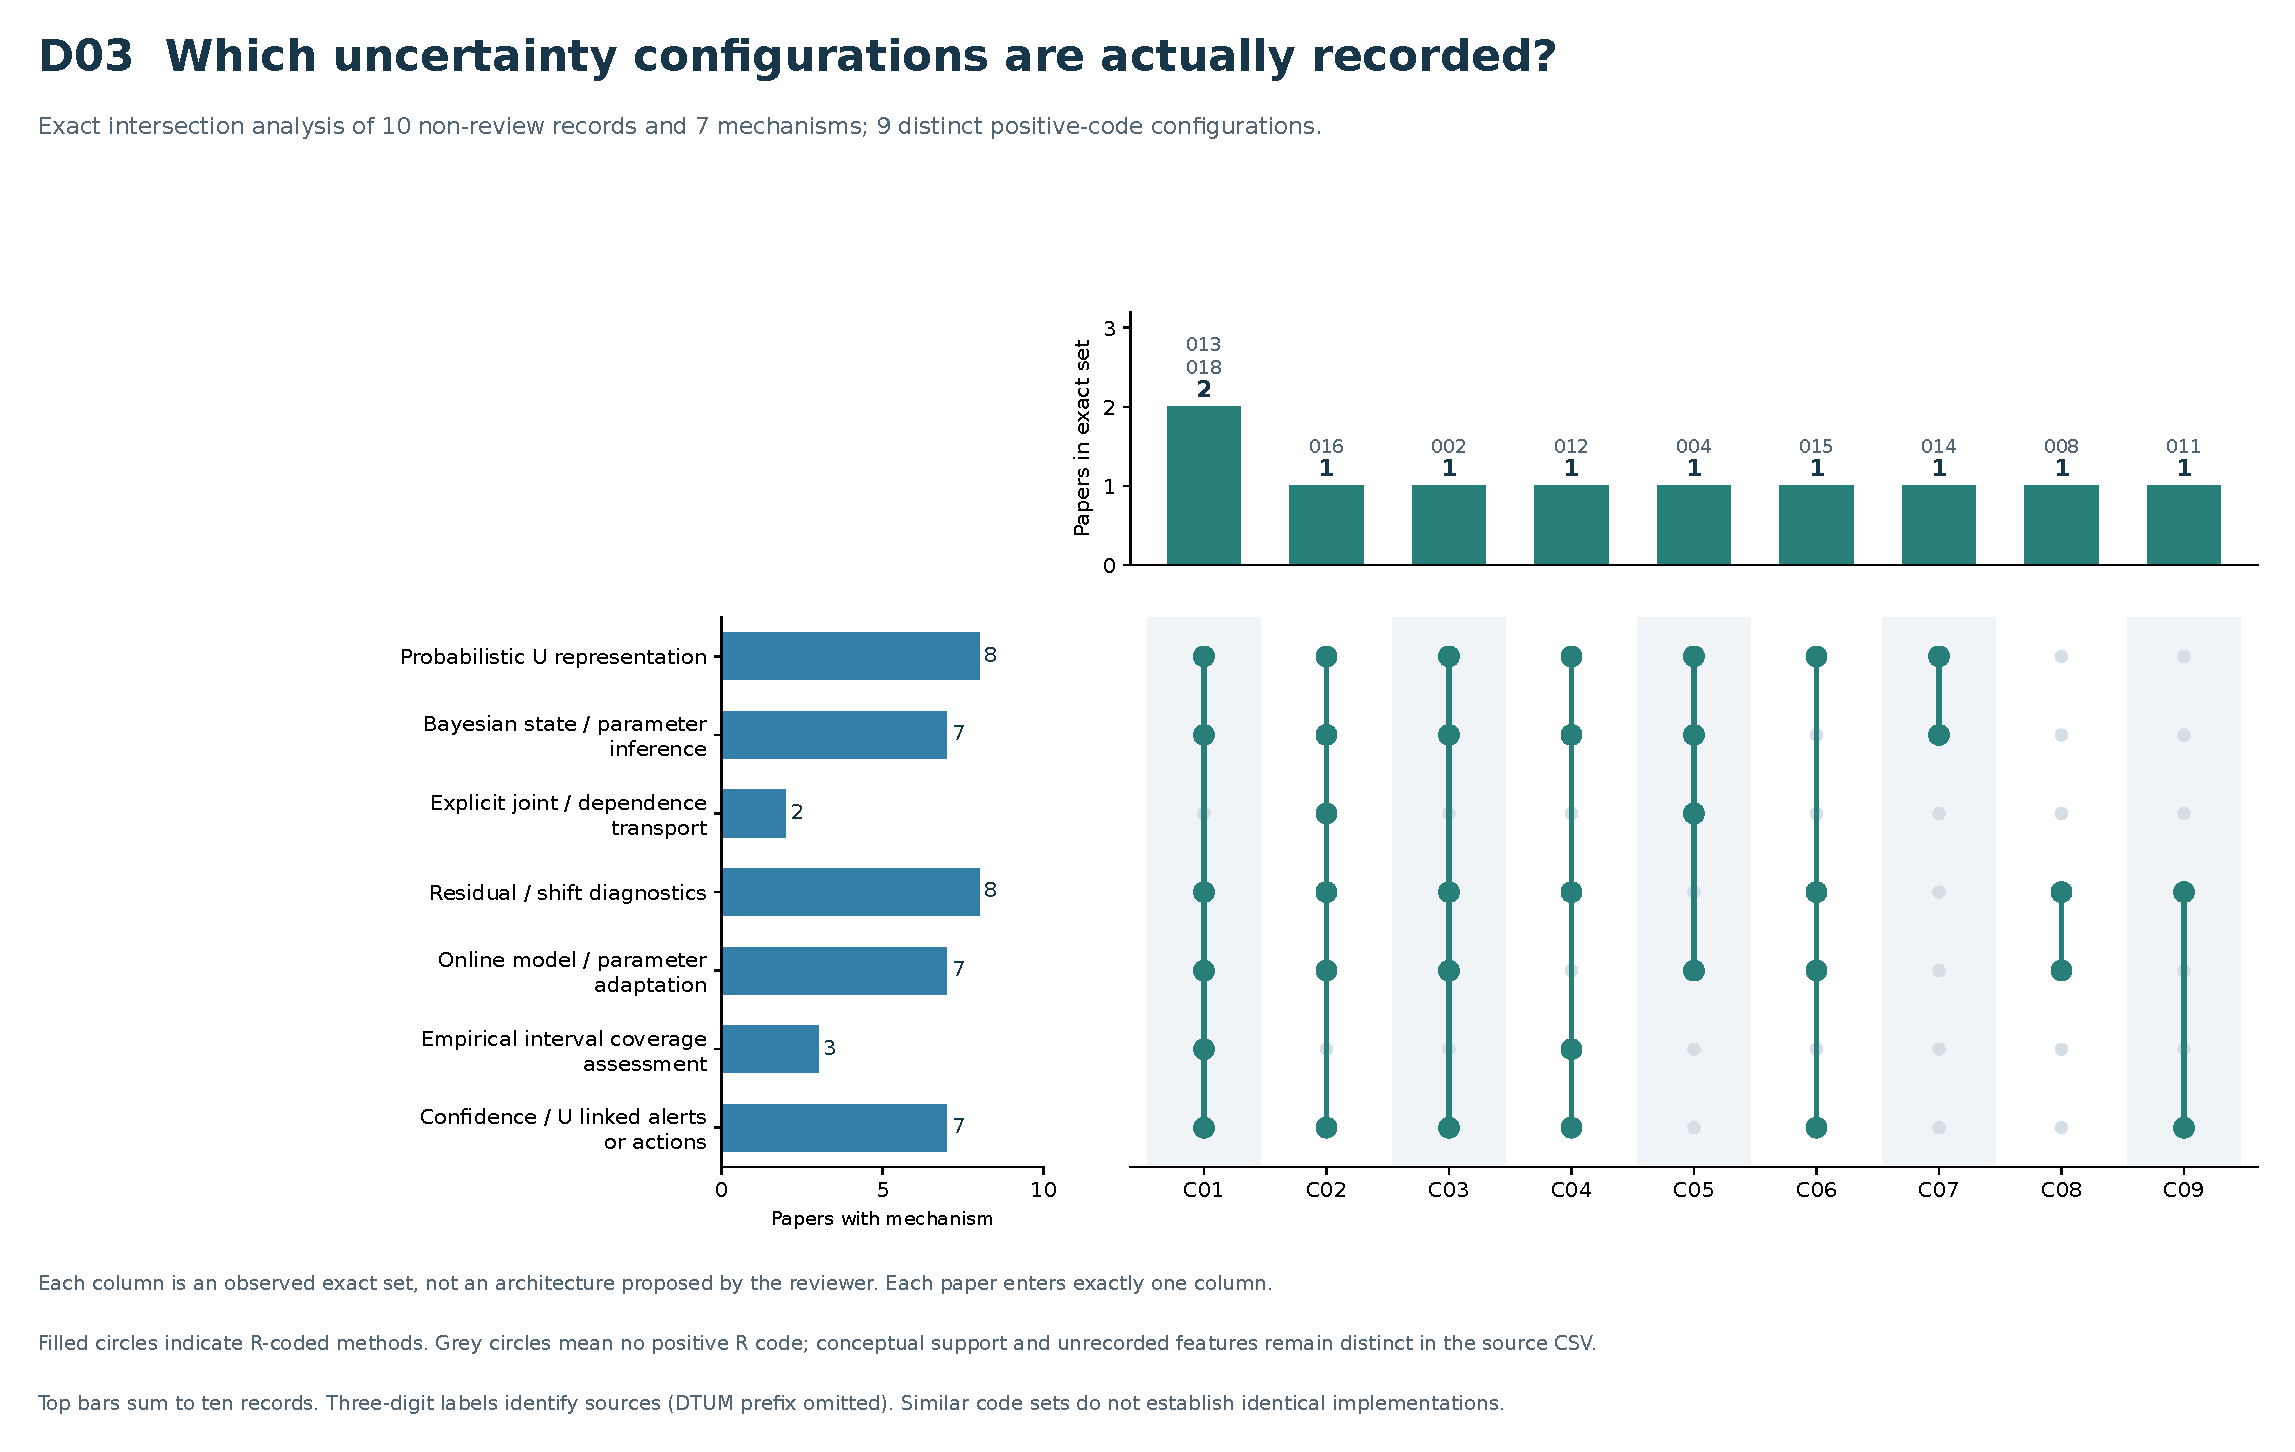
\includegraphics[width=\linewidth,height=.82\textheight,keepaspectratio]{../../relational_analysis/data_diagrams/figures/D03_exact_uncertainty_configurations.pdf}\caption{Exact positive-code intersections. Each publication occupies one configuration.}\end{figure}
The source–method matrix provides a bridge between these observations. It contains 46 positive cells among 100 possible source–method cells. For geometry-related contexts, sensitivity/comparison and prediction diagnostics each occur in 3/8 contexts (37.5\%). For lifetime/timing contexts, sensitivity and range/distribution representation each occur in 4/8 (50.0\%). Scenario comparison accompanies future-scenario sources in 4/5 contexts (80.0\%). The recovery source has only one assessed context, associated with sampling and scenario comparison. These are same-publication, same-context associations; they do not establish that every paired method was specifically applied to every paired source.

\begin{figure}[p]\centering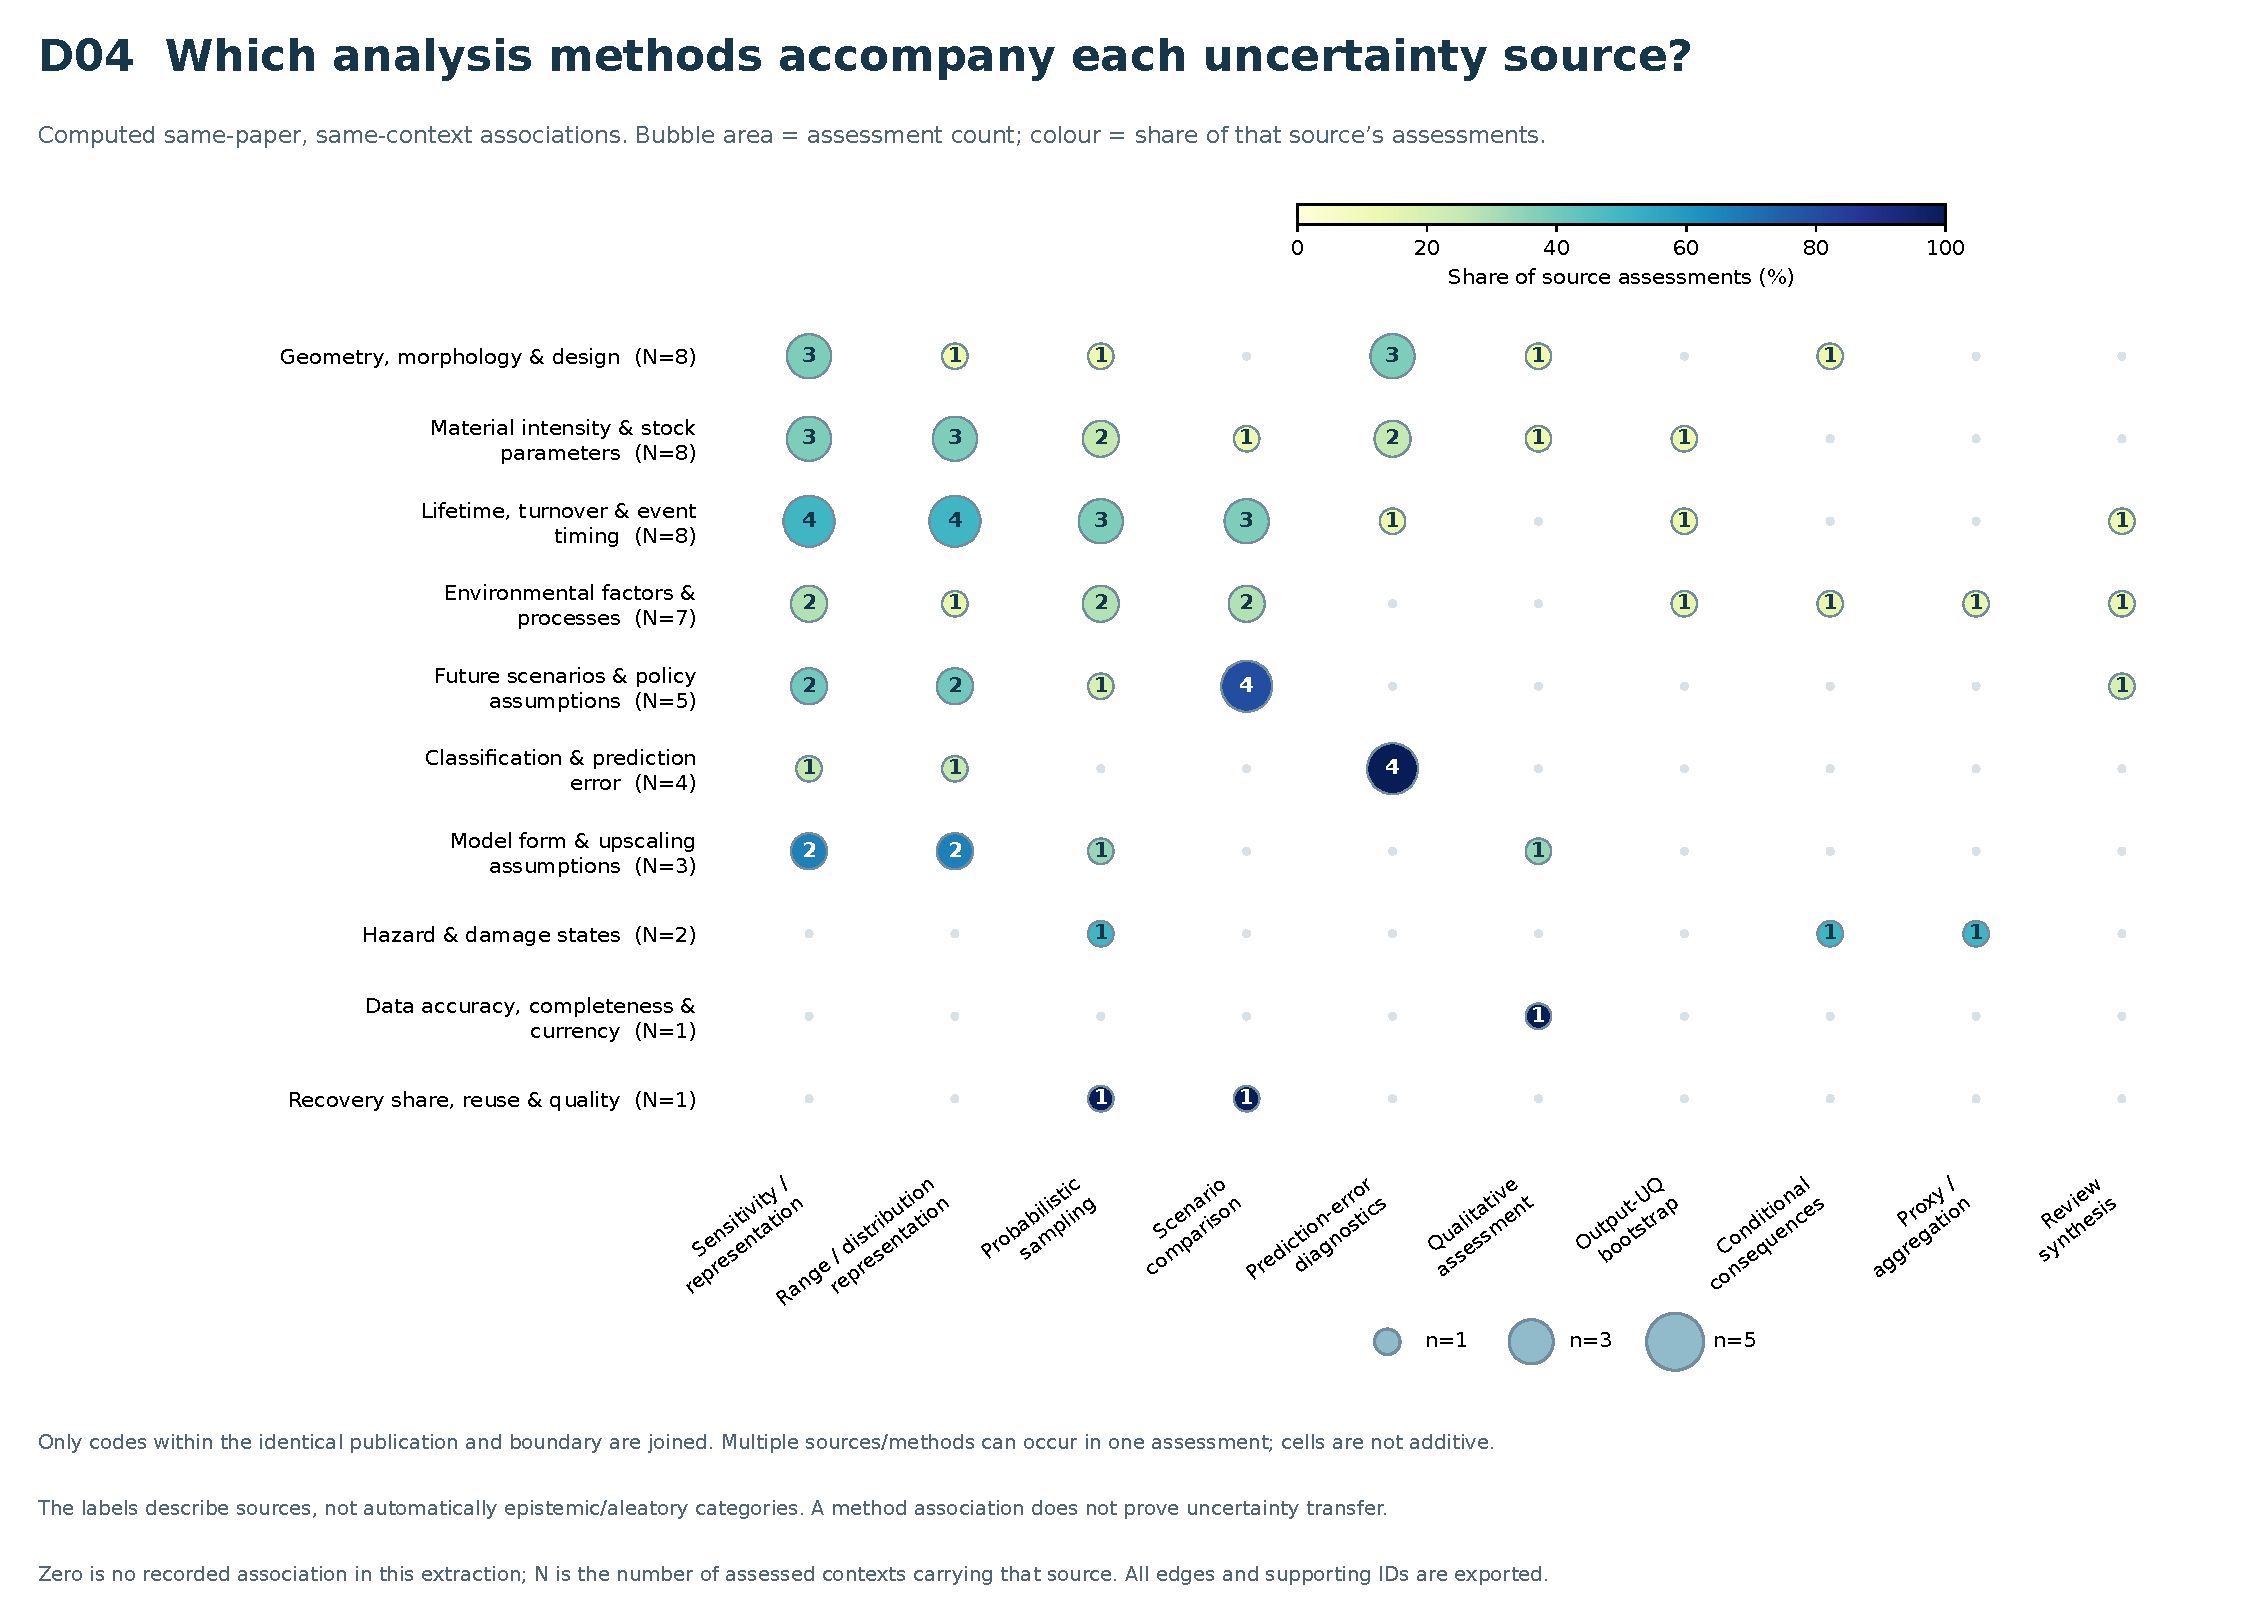
\includegraphics[width=\linewidth,height=.82\textheight,keepaspectratio]{../../relational_analysis/data_diagrams/figures/D04_uncertainty_source_method_associations.pdf}\caption{Source–method co-occurrence restricted to the same paper and context.}\end{figure}
\subsection{From configuration descriptors to an uncertainty-traceable architecture}
The supplied DT design framework contributes three complementary questions. The design brief specifies what the representation is for. Configuration describes how models, services, information and interactions are arranged. Functional allocation identifies where calibration, evaluation, prediction and decision activities are performed. The literature supports several underlying concepts, but the A–B–C organisation and the complete arrangement are a synthesis, not a taxonomy statistically recovered from the selected papers \citep{R1,R2,R5,R6}.

\begin{figure}[p]\centering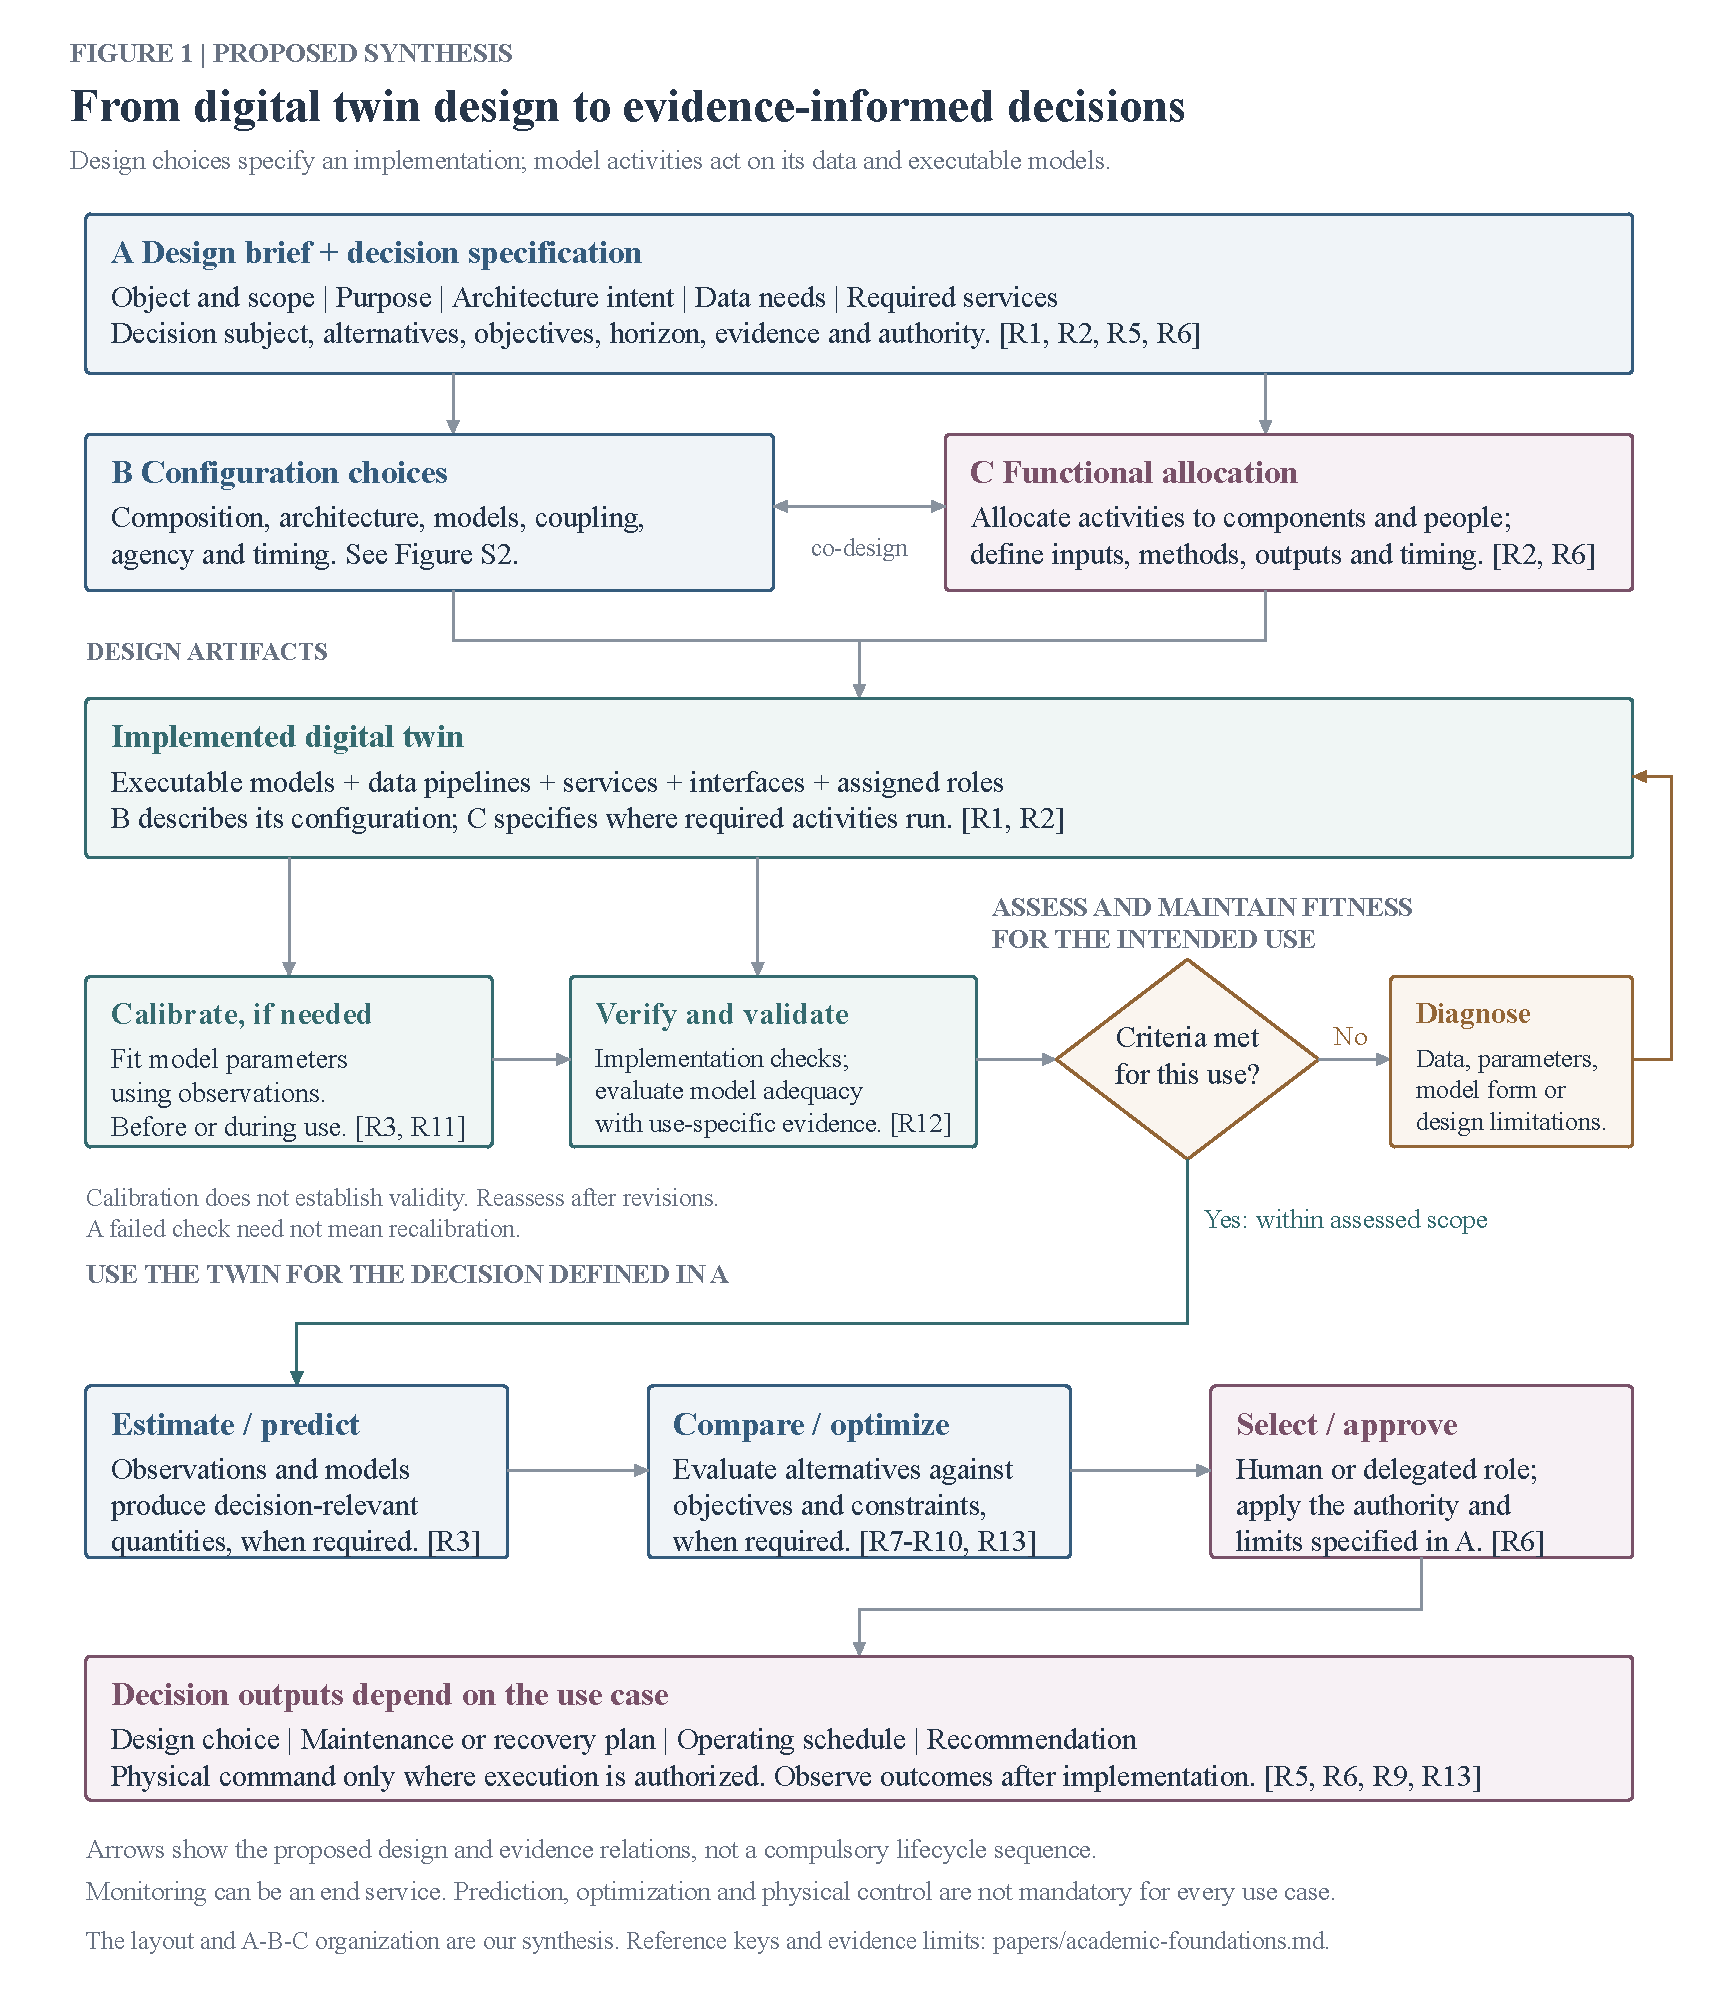
\includegraphics[width=\linewidth,height=.82\textheight,keepaspectratio]{../inputs/figure_1_design_to_use.pdf}\caption{Previously developed design-to-use synthesis. R keys are resolved in the accompanying foundations register; arrows are conceptual.}\end{figure}
Configuration descriptors are not uncertainty parameters. For example, a hybrid model combines modelling bases, but does not by itself quantify model discrepancy. A knowledge graph can preserve identity and relationships, but does not automatically propagate a joint distribution. A federated architecture can connect services, but requires an explicit interface contract to preserve units, time references and dependency information. Likewise, bidirectional data exchange is distinct from autonomous authority. The configuration diagram is therefore used to identify implementation choices that could support required functions; its curves are not counted as observed connections \citep{R14,R15}.

\begin{figure}[p]\centering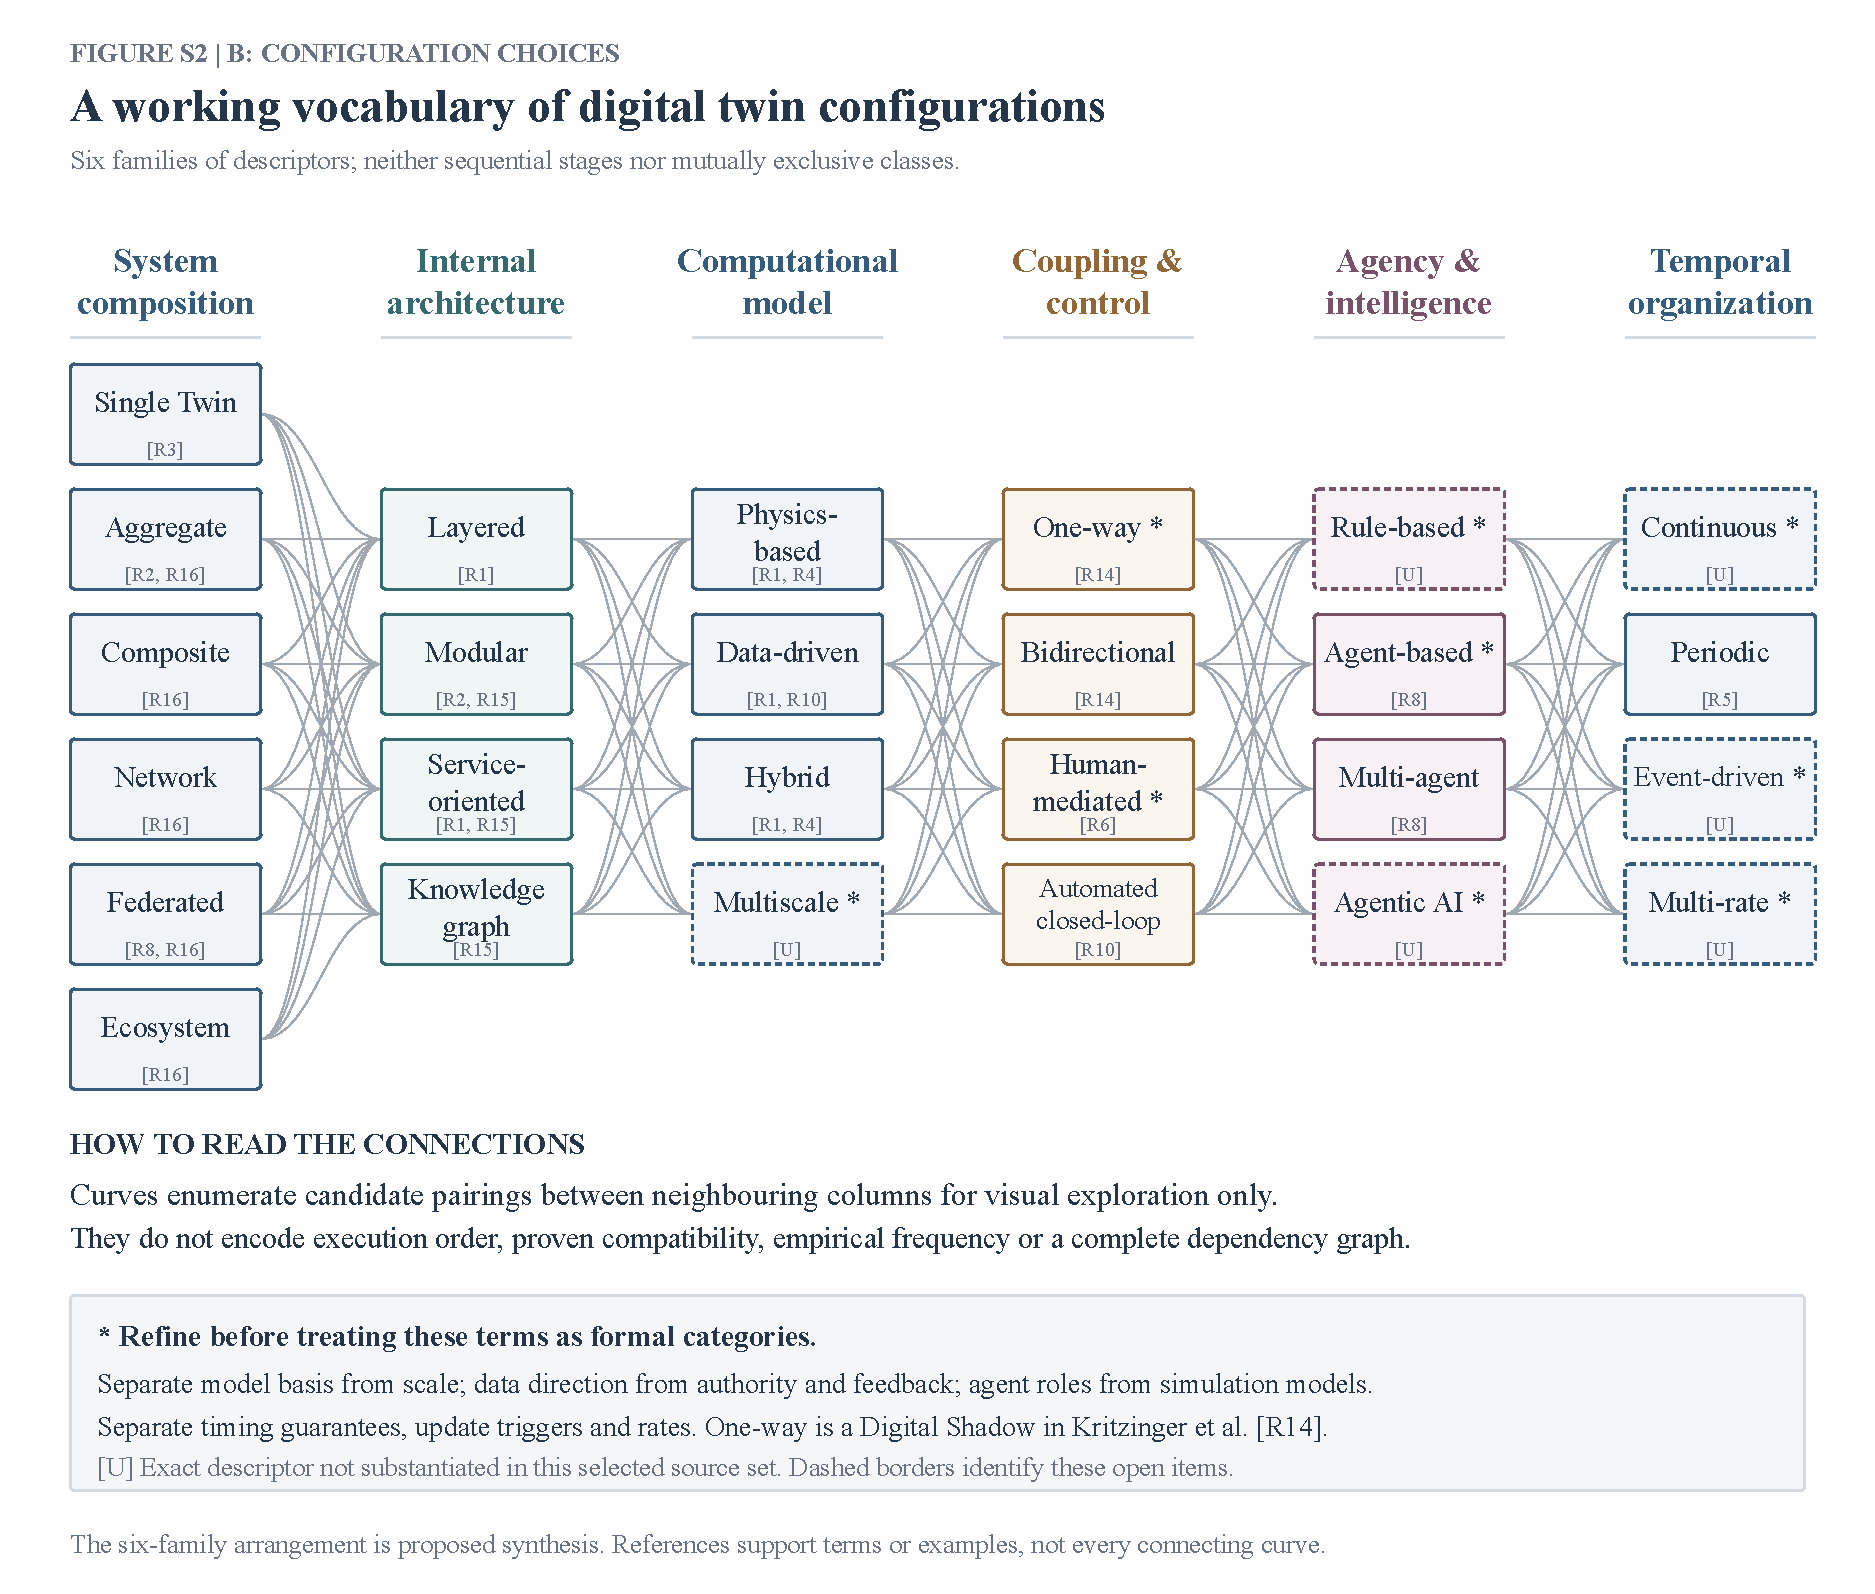
\includegraphics[width=\linewidth,height=.82\textheight,keepaspectratio]{../inputs/figure_S2_configuration_choices (1).pdf}\caption{Configuration vocabulary, not empirical pair frequencies. Unresolved terms remain marked in the original figure.}\end{figure}
The transition-centred synthesis adds a shared record to these design choices. For each transferred material variable, it records identity, value and unit, uncertainty representation, dependencies, transformation, spatial support, valid time, model version, supporting evidence and decision use. This record is the proposed means of keeping continuity inspectable across heterogeneous models. The following parameters define its operational meaning; they are synthesis requirements rather than measured results of a deployed system.

\begin{longtable}{p{5.17cm}cm}cm}}
Parameter & Operational definition & Relevance to uncertainty tracking\\
Entity and variable identifier & Stable reference to building, component, material batch and quantity & Prevents mismatching observations, stocks and recovery outputs\\
Value, unit and spatial support & Quantity plus its physical unit and represented spatial extent & Makes conversions and aggregation explicit\\
Valid time and version & Time represented by the datum; model/data version; update time & Distinguishes real change from asynchronous or stale information\\
Uncertainty representation & Distribution, samples, interval, scenarios or qualitative statement & Prevents replacement by an unexplained point value\\
Dependency information & Joint samples, covariance or conditional relations, where supported & Preserves correlated inputs and avoids unjustified independence\\
Transformation identifier & Mapping f, parameters, assumptions, output variable and unit & Identifies where uncertainty changes meaning or scale\\
Observation and residual & Independent observation and difference from prediction, with noise model & Detects disagreement; does not uniquely identify its cause\\
Coverage and sharpness & Empirical interval coverage and interval width in a stated evaluation set & Tests reliability of uncertainty estimates, rather than accuracy alone\\
Update rule and trigger & What information changes which state/parameter and when & Makes uncertainty revision traceable\\
Decision threshold and authority & Action criterion, tolerance and authorised role & Connects uncertainty to decisions without assuming automatic control\\
Evidence and support class & Paper, page/table, and direct, synthesised or proposed status & Makes the architectural claim auditable\\
\end{longtable}
\begin{figure}[p]\centering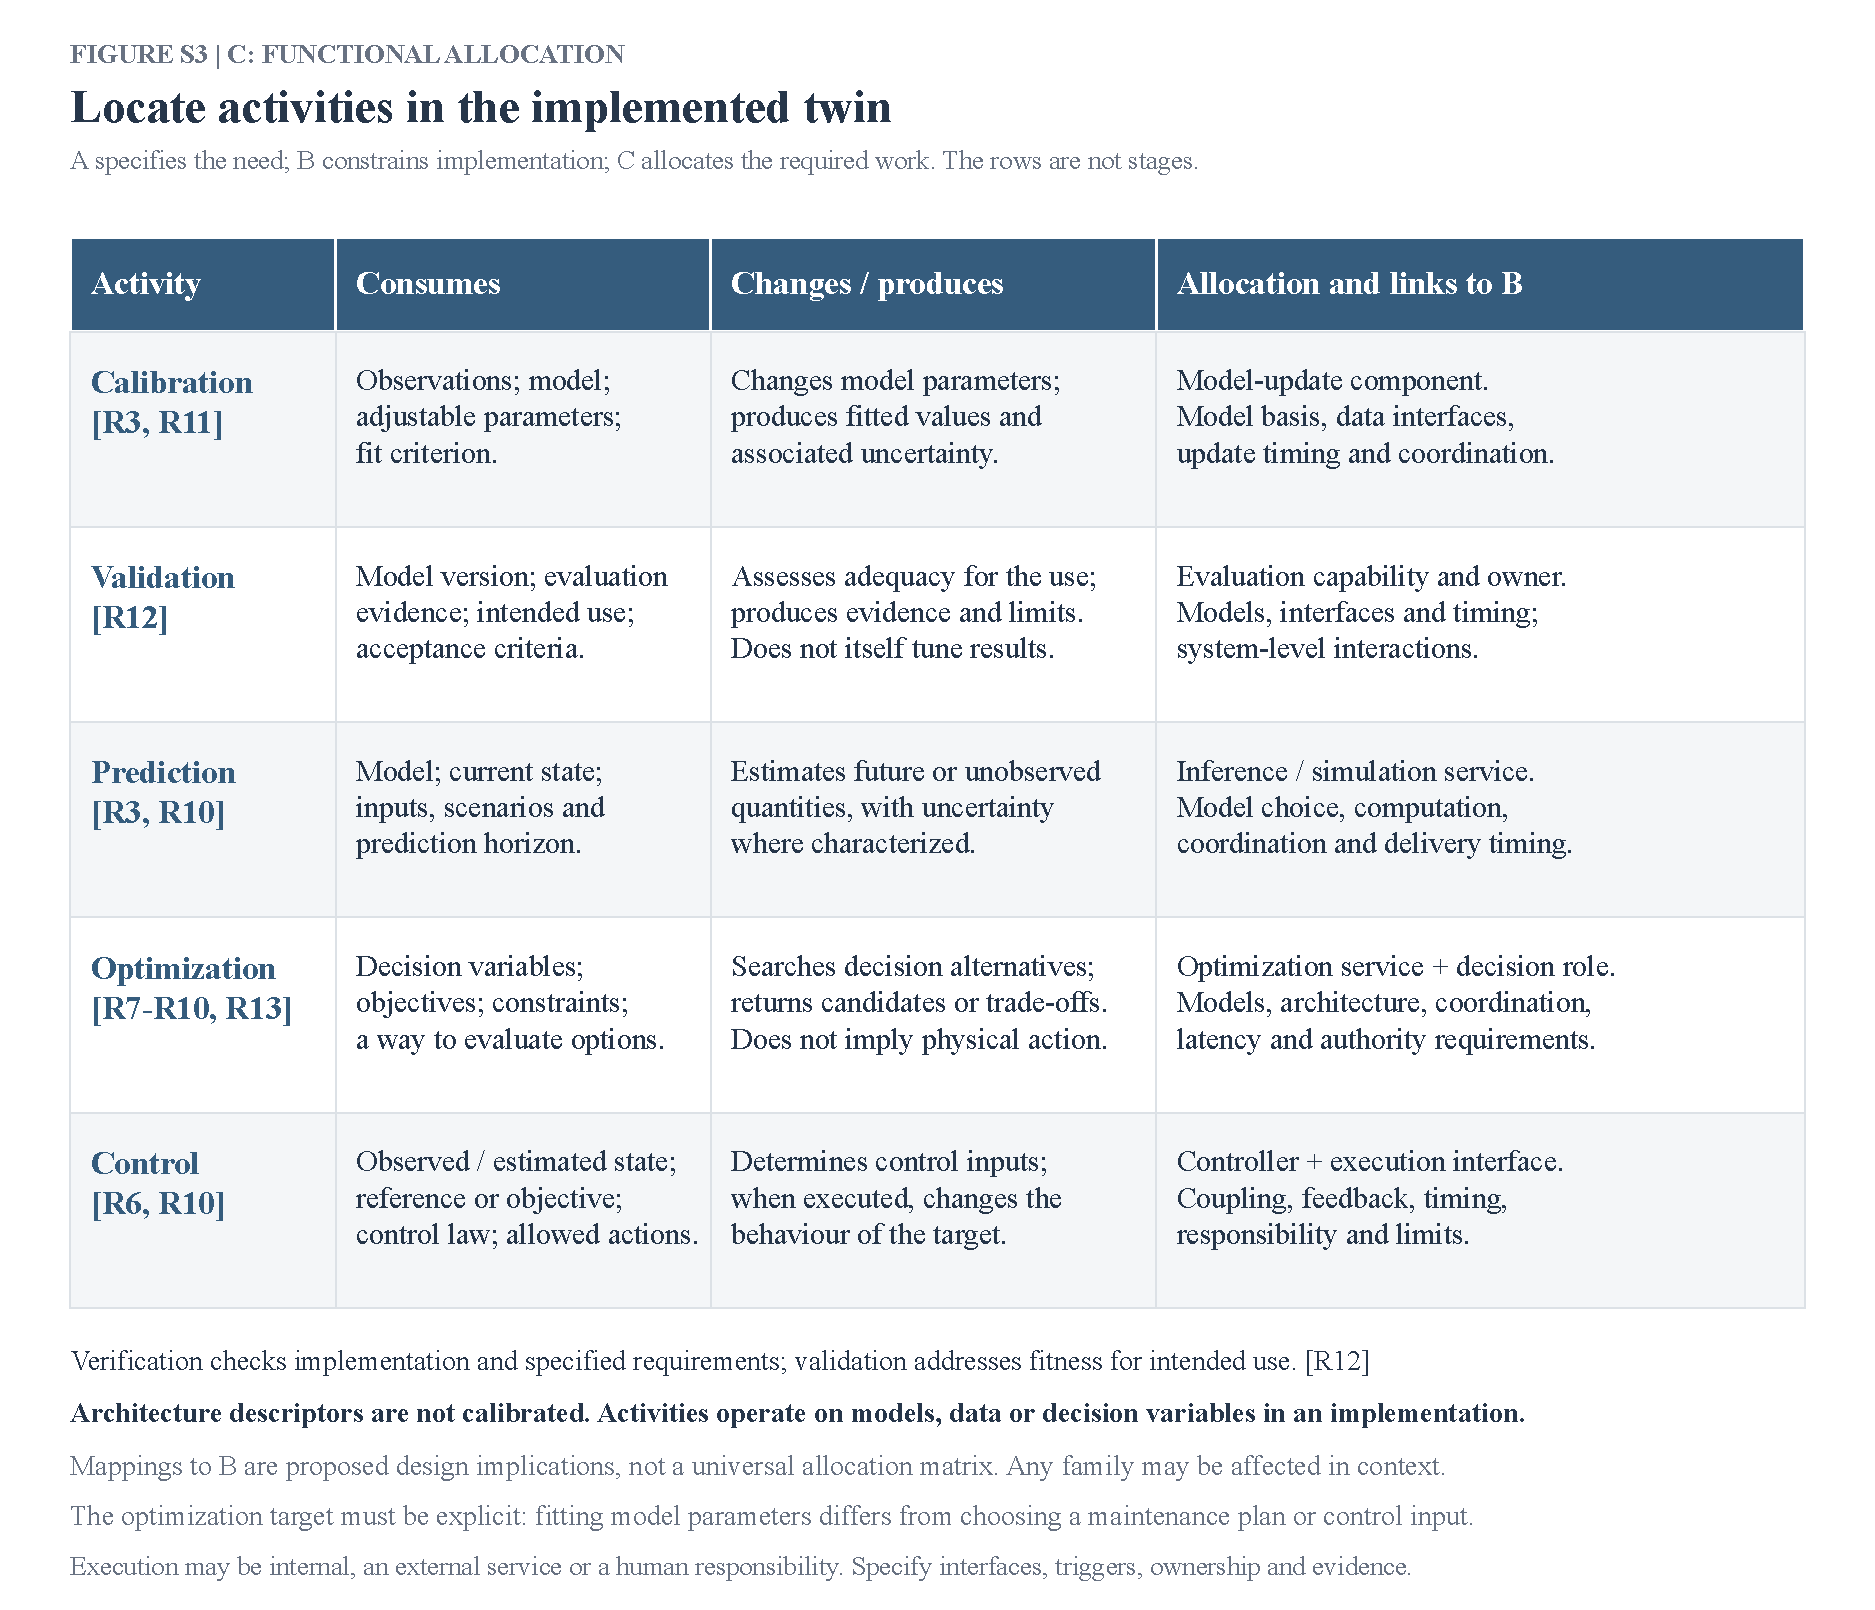
\includegraphics[width=\linewidth,height=.82\textheight,keepaspectratio]{../inputs/figure_S3_functional_allocation.pdf}\caption{Functional allocation. Activities are not equivalent to material-flow stages.}\end{figure}
This synthesis identifies places where uncertainty can become observable to the user of the twin: input-quality checks, state inference, cross-model propagation, predictive diagnostics and decision evaluation. The architecture does not discover every unknown source automatically. It can expose failures of specified assumptions and information contracts, while unmodelled mechanisms require further investigation. The proposed deployment of these functions at all four material-flow boundaries remains an architectural response to the reviewed evidence, not a demonstrated end-to-end implementation.

\begin{figure}[p]\centering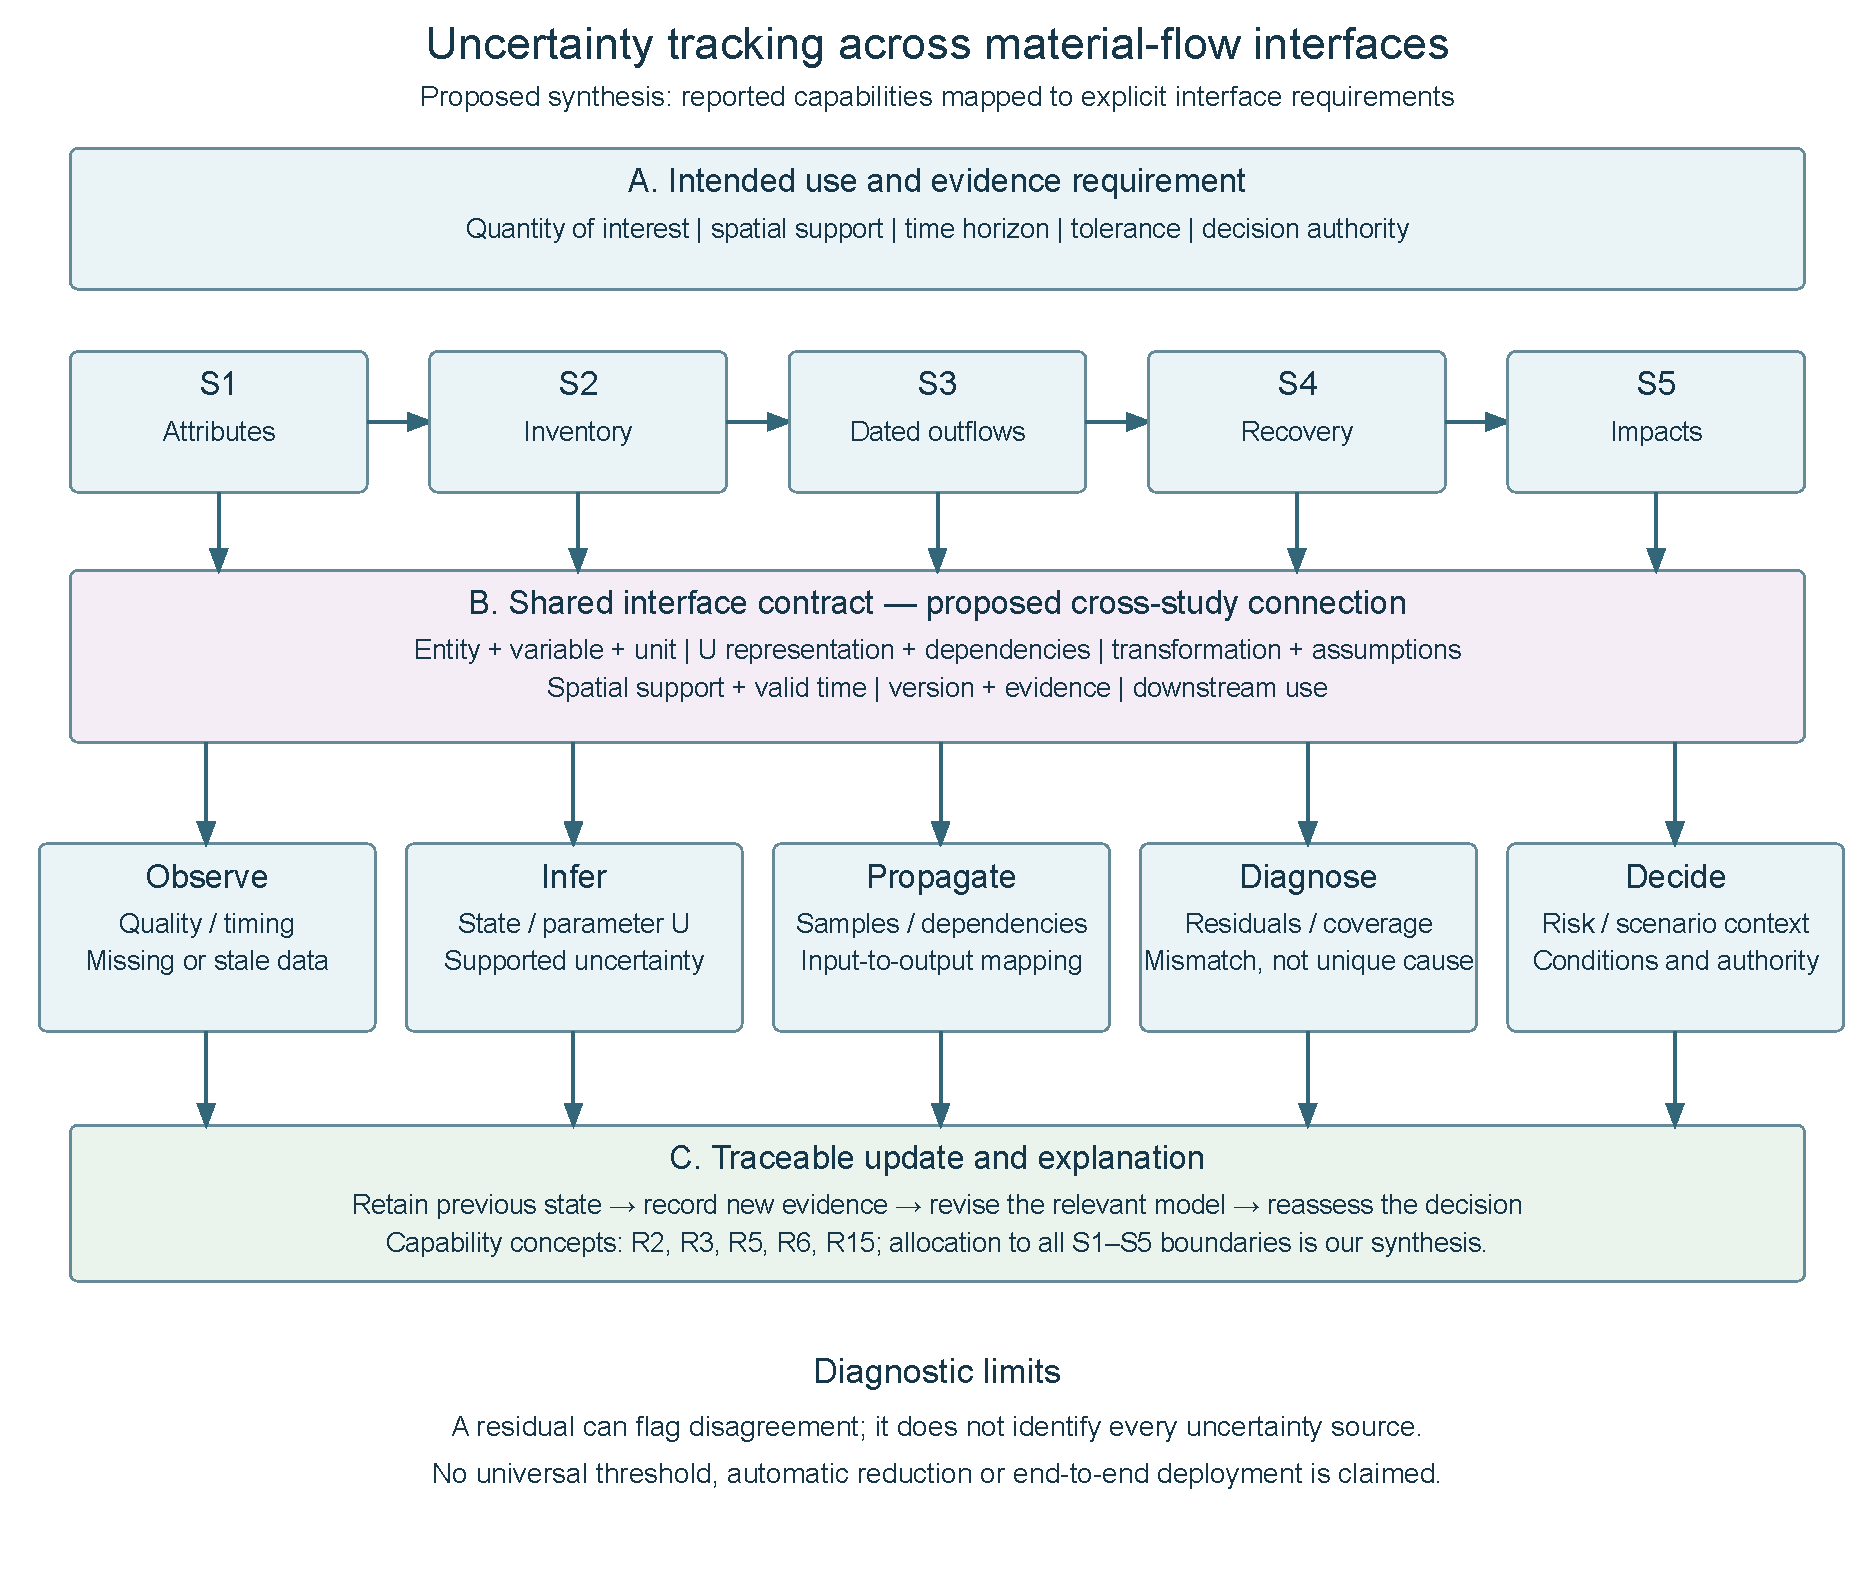
\includegraphics[width=\linewidth,height=.82\textheight,keepaspectratio]{../figures/F07_tracking_architecture.pdf}\caption{Proposed uncertainty-tracking overlay. Capability concepts have literature support; complete interface allocation is synthesis.}\end{figure}
\section{Discussion}
\subsection{Continuity is a property of interfaces, not the presence of UQ software}
The central implication is that uncertainty-aware components do not automatically form an uncertainty-continuous workflow. GeoAI can produce an error score, a stock model can use variable material coefficients, and a lifecycle model can run Monte Carlo, yet these activities may refer to different uncertain inputs. The review therefore shifts the question from whether a method appears in a paper to whether the information needed by the next transformation survives the interface. Integrated stock–flow and impact workflows motivate this question, while the transition analysis specifies how it can be examined \citep{U01,I35,I36,I37}.

Three operations must be distinguished. Propagation computes consequences of specified uncertain inputs. Updating changes an uncertainty representation in light of observations or revised assumptions. Validation evaluates whether predictions and their uncertainty are adequate for the intended use. Running one operation does not establish the other two. In particular, a small prediction error does not establish calibrated predictive intervals, and a narrower posterior does not establish that missing mechanisms have been resolved. A digital twin is useful here because it can organise repeated observation, model revision and evidence evaluation, provided these operations are implemented explicitly \citep{I33,R5}.

\subsection{What must cross each material-flow boundary?}
At S1→S2, the transformation links inferred building attributes to material quantities. A schematic stock calculation is M = Σ\_b A\_b I\_b, where A denotes a relevant geometric measure and I a compatible material-intensity coefficient. The uncertainty of the product depends on both factors and their dependence. Transferring only the predicted building class or mean coefficient loses information needed by the inventory model. A useful DT interface would retain class probabilities or alternative attribute states, material-coefficient uncertainty, consistent units and the aggregation rule. It should not turn a classification confidence score into a calibrated probability without supporting evaluation.

At S2→S3, an inventory is transformed into dated outflows using age, lifetime, renovation and event assumptions. A schematic mapping O(t) = Σ\_c M\_c f\_c(t | age, scenario) emphasises that the output is a flow in a time interval rather than a stock at a date. The uncertainty representation must therefore carry material quantities together with the event-time model. A new building survey can update stock information, while a renovation event may revise remaining life and outflow timing. Revisions must preserve their relationship to the previous state rather than silently overwrite the forecast \citep{U11,U12,U13,U18}.

At S3→S4, potential outflow becomes technically recoverable and route-specific material. R = O × η × q is a deliberately schematic expression: η represents yield and q a quality/acceptance factor, and their meanings must be defined for the selected reuse or recycling route. Damage, contamination and selective-disassembly evidence may change these factors and their dependence. The current absence of a coded context at this boundary makes a condition-observation and recovery-evaluation interface a justified research priority, but not a validated solution. It would be inappropriate to assign universal recovery distributions to fill that gap \citep{I20,I21}.

At S4→S5, recovered materials acquire environmental consequences under substitution, allocation and system-boundary assumptions. A schematic impact calculation sums route-specific material quantities multiplied by environmental factors and subtracts eligible avoided burdens. The same recovered mass can lead to different results when substituted products, quality equivalence or future energy systems differ. A traceable interface must retain those conditions along with material quality and quantity. Circularity alone does not establish an environmental benefit, and a reported impact interval cannot be interpreted as end-to-end uncertainty unless upstream recovery uncertainty is included \citep{U19,I22,I38}.

These expressions illustrate interface requirements; the review has not fitted or executed a combined material-flow model. Their role is to make the architectural requirements precise enough for subsequent empirical testing.

\subsection{How the twin could detect, track and explain uncertainty}
The proposed architecture uses a common evidence contract across the four boundaries and allocates different checks to the functions that can perform them. The observation service checks completeness, calibration, coverage and timing. The inference service estimates states or parameters and records posterior or other supported uncertainty. The propagation service passes compatible samples, distributions or scenario identifiers through a stated transformation. The diagnostic service compares predictions with independent observations. The decision service expresses the consequences of the remaining uncertainty for an authorised choice. Identity, provenance and versions connect these services, while stakeholder roles determine who may revise assumptions, approve evidence or act on outputs \citep{R2,R6,R15}.

A useful diagnostic is a residual r = y\_observed − y\_predicted. A persistent or unexpectedly large residual can indicate a problem, but may originate in measurement noise, stale input, parameter error, model discrepancy or changed conditions. Diagnosis therefore requires assumptions about both observation and prediction. Under an appropriate predictive model, a standardised residual may divide r by the square root of predictive plus observational variance, including dependence terms where relevant. Such a diagnostic must not be presented as a universal detector or given an arbitrary threshold.

Tracking requires more than storing successive uncertainty widths. A change from a stock interval in tonnes to an impact interval in kilograms CO2-equivalent is a transformation in quantity and unit. Directly comparing the numerical variances would be meaningless. Comparisons of amplification or reduction require a common quantity, compatible scale and context, or a stated normalisation. Likewise, aggregation can reduce relative variability when errors offset while preserving a shared bias. These distinctions explain why the outcome sketches are a conceptual vocabulary, not numerical results for each stage.

The uncertainty representation should remain plural. Sampling or Bayesian inference is useful when probabilistic assumptions are supported; scenario comparisons remain appropriate when future alternatives do not have defensible probabilities. A qualitative limitation should be carried as a limitation rather than assigned an invented distribution. This allows a stakeholder to see both the calculated uncertainty and what the calculation has left outside its scope \citep{I25,I33}.

\subsection{Architectural synthesis, scale and decision relevance}
The novelty of the review lies in connecting three bodies of evidence through explicit interface requirements: material-flow uncertainty, domain-specific DT functions and general DT uncertainty mechanisms. It does not lie in inventing a new estimator, implementing a universal twin or demonstrating a reduction in environmental uncertainty. Direct evidence supports particular functions; compatibility reasoning links functions from different studies; proposals identify what still needs to be tested. The full architecture consequently remains a literature-informed, evidence-traceable synthesis.

The A–B–C design structure helps avoid treating every digital twin as the same technical object. A purpose such as stock estimation requires different observation frequency and validation evidence from an imminent recovery decision. A city-scale model and a component-level reuse assessment can share a record structure while requiring different spatial support, identifiers, uncertainty dependencies and validation data. This makes the design adaptable across scales; it does not establish scale-independent validity or computational scalability \citep{R1,R5}.

Stakeholders enter the architecture through information needs, authority and evidence responsibilities rather than a fixed list of organisations. Timing enters through valid time, update time, event triggers and decision horizon. A periodic or event-driven update can be suitable when the represented material state changes slowly; fast synchronisation alone cannot compensate for poor material information. The decision interface should report the quantity of interest, uncertainty representation, scenario conditions, evidence status and the reason for any recommendation \citep{R5,R6}.

\subsection{Limits and research priorities}
The strongest quantitative statements in this draft are reproducible frequencies within named coding sets. The archival 17-paper analysis and current 20-paper context analysis use different coding schemes and must not be combined as repeated samples. The former includes secondary and supporting-information-based evidence; the current eligibility ledger contains later targeted full-text checks, but does not retroactively establish every legacy outcome label. The general-DT subset is small and cross-domain. None of these distributions supports a population prevalence estimate or a ranking of uncertainty methods by effectiveness.

No pooled percentage reduction in uncertainty is reported. Such a synthesis would require extracting the quantity of interest, units, probabilistic assumptions, sample or scenario basis, uncertainty metric, upstream/downstream comparison and validation conditions from each eligible primary study. RMSE, coefficient of variation, confidence intervals, prediction intervals and scenario ranges cannot be pooled merely because all describe some form of spread or error. The existing extraction does not provide a harmonised basis for that operation.

The next empirical test should focus on one fully documented boundary before attempting the entire chain. It should compare deterministic transfer with a dependency-preserving alternative, retain identical input evidence, evaluate held-out observations where available, and test how changes affect the decision rather than interval width alone. Particular priority belongs to S3→S4 and to the connection between recovery quality and environmental substitution. Completing pending eligibility and page-specific evidence reconciliation remains necessary before this working manuscript can be submitted as a closed systematic review.

Taken together, the analyses suggest a precise role for digital twins: maintaining an inspectable relationship between uncertain observations, model transformations and decision consequences over time. The review supports this as an architectural direction, while leaving its end-to-end performance to future validation.
